\listfiles
\documentclass[fontsize=11pt,%            % corpo del font principale
               a4paper,%                  % formato carta A4
               twoside,%                  % fronte-retro
               openright,%                % apertura capitolo a fronte
               titlepage,%                % frontespzio
               fleqn,%                    % equazioni allineate a sinistra
               headinclude=true,%         % testatina
               footinclude=true,%         % pie' di pagina
               BCOR5mm,%                  % rilegatura di 5 mm
               numbers=noenddot,%         % niente punto dopo il numero sez
               cleardoublepage=empty,%    % pagine vuote senza testatina etc
               %tablecaptionabove,%       % didascalie in cima alle tabelle
               captions=tableheading,%    % didascalie in cima alle tabelle
               version=first,english,%
               abstracton%
               ]{scrreprt}                % classe report di KOMA-Script;
               
% *****************************************************************************
% classicthesis-preamble
% *****************************************************************************

\newcommand{\myName}{Alessandro Candolini}
\newcommand{\myTitle}{Statistical Data Analysis }
\newcommand{\mySubTitle}{Theory, methods, algorithms and modern techniques\\
   from high-energy and computational physics to information technology}
\newcommand{\myDegree}{}%Tesi di laurea}
\newcommand{\myUni}{University of Trieste}
\newcommand{\myFaculty}{Facolt\`a di Scienze Matematiche, Fisiche e Naturali}
\newcommand{\myDepartment}{Department of Theoretical Physics}
\newcommand{\myProf}{Chiar.mo Prof.~S.~Anselmo d'Aosta}
\newcommand{\myLocation}{Trieste}
\newcommand{\myTime}{\today}

% *****************************************************************************
%  Main packages
% *****************************************************************************

\usepackage[english]{babel}       % Attiva supporto per la lingua.
\usepackage[babel]{csquotes}              % Consigliato se si usa biblatex.

\usepackage{graphicx}                     % Per le immagini.

\usepackage{mparhack}                     % Get marginpar right.
\usepackage{fixltx2e}                     % Fixes some LaTeX stuff.
\usepackage[final]{microtype}             % Microgiustificazione e finezze.

%\usepackage[tight,english]{minitoc}       % Mini-indici a inizio capitolo.
\usepackage{mtcoff}

\usepackage{wrapfig}                      % Figures which text can flow around.
\usepackage{chngpage,calc}                % Per impostare i margini del
					  % Frontespizio.

\usepackage{mflogo}                       % Support for Metafont logo fonts.
\usepackage{listings}                     % Ambienti per listati di codice.
\usepackage{ifpdf}                        % To check if pdflatex is used.

\ifpdf
  \DeclareGraphicsRule{*}{mps}{*}{}       % To include metapost files.
\fi

\usepackage{multicol}                     % Supporto per piu' colonne
\usepackage{makeidx}                      % Supporto per l'indice analitico.


\usepackage{subfig}                       % Multiple figures.
\usepackage{url}                          % Url.
\usepackage{hyperref}                          % Url.

% *****************************************************************************
% Quoting 
% *****************************************************************************

\usepackage[font=small, noorphanfirst,
indentfirst=false,
%begintext=\openautoquote,
%endtext=\closeautoquote,
]{quoting}         

% *****************************************************************************
% BIBLaTeX
% *****************************************************************************
%\usepackage[%
%style=philosophy-modern,%
%%style=philosophy-classic,%
%%style=philosophy-verbose,%
%scauthorsbib,%
%%hyperref,backref,%
%backend=biber,
%square,%
%ibidtracker=true]{biblatex}

\usepackage[%
%%refsection=chapter,%
autocite=footnote,%
autopunct=false,%
%%style=philosophy-modern,%
style=philosophy-verbose,%
publocformat=publocyear,%
%%shorthandintro=false,
scauthorsbib,%
scauthorscite,
backend=biber,
dashed=true,
singletitle=true,
firstinits=true,%
origfields=trans,%
origfieldsformat=semicolon,%
latinemph=true,%
commacit=false,%
hyperref=true,%
backref=true,%
%publocformat=loccolonpub,%
%volumeformat=romanscRoman,%romansc,romanupp
editionformat=arabic,%romansc,%roman,%romansc,romanupp
annotation=true,
library=true,
pagetracker=true,
opcittracker=true,
uniquename=true,%
isbn=false,%
%indexing=cite
]{biblatex}
  
\addbibresource{myBibliography9.bib}            % database di biblatex 



% *****************************************************************************
% ClassicThesis 
% *****************************************************************************
\PassOptionsToPackage{small}{eulervm}%
\PassOptionsToPackage{euler-hat-accent}{eulervm}%
\PassOptionsToPackage{loosequotes}{MinionPro}
\PassOptionsToPackage{footnotefigures}{minionpro}
\usepackage[eulerchapternumbers,%         % Numeri dei capitoli in Euler.
            listings,%                    % Se si vuole  inserire listati.
            pdfspacing,%                  % Miglior riempimento di linea.
            floatperchapter,%             % Numerazione float per capitolo.
            subfig,%                      % Compatibilita' con subfig.
            beramono,%                    % Bera Mono font a spaziatura fissa.
            eulermath,%                   % AMS Euler come font per matematica
            parts,                        % Per documenti suddivisi in parti.
            minionpro%                    % Usa Font Minion Opticals.
            ]{classicthesis}              % Lo stile ClassicThesis

\usepackage[eqno,toc,enum,bib]{tabfigures}% Per numerazione.

%\usepackage{arsclassica}                  % Modifica aspetti di ClassicThesis


% *****************************************************************************
% 	General commands
% *****************************************************************************

% [...] ;-) NO replaced by \textelp{} and other feature of cvsquotes package
%\newcommand{\omissis}{[\dots\negthinspace]}

% Indica a LaTeX la cartella dove sono riposti i file delle immagini
\graphicspath{{./},{./Asymptote/}, {./Images/}, {./Metapost/}}

% Un ambiente ad hoc per gli approfondimenti (definirlo si, ma magari in altro
% modo)
\newenvironment{approfondimento}%
{\begin{quoting}}
  {\end{quoting}}

% i.e. and e.g.
% here with thin space (most german convetion), see typography discussion in 
% http://tex.stackexchange.com/questions/25831/canonical-way-to-typeset-spacing-in-abbreviations
\providecommand{\ie}{i.\,e.}
\providecommand{\Ie}{I.\,e.}
\providecommand{\eg}{e.\,g.}
\providecommand{\Eg}{E.\,g.} 

% th
\newcommand{\ordth}{\textsuperscript{th}}

% Cpp 
\def\cpp{\mbox{C++}}

% *****************************************************************************
% 	Signature
% *****************************************************************************
% tmark 
\newcommand{\tmark}[1]{%
  {{\unskip\nobreak\hfil\penalty50
  \hskip2em\vadjust{}\nobreak\hfil[#1]%
  \parfillskip=0pt \finalhyphendemerits=0 \par
  \penalty 10000 \parskip=0pt\noindent}}\ignorespaces}

% Signature environment
\makeatletter
\newcommand*{\stopbreaks}{%
  \interlinepenalty\@M
  \def\par{\@@par\nobreak}%
  \let\\\@nobreakcr
  \let\vspace\@nobreakvspace}
\makeatother

\def\signature{%
  \par\raggedleft\nopagebreak\vspace{.8em}%
%  \stopbreaks%
}
\def\endsignature{\par}%\endgroup\par}

\newcommand{\mySignature}[2]{%
  \par\noindent\nopagebreak\vspace{.8em}%
  \begingroup
  \stopbreaks%
  \begin{minipage}[b]{0.49\textwidth}%
  \raggedright
  #1
  \end{minipage}
  \hfill
  \begin{minipage}[b]{0.49\textwidth}
  \raggedleft
  #2
  \end{minipage}
  \endgroup
  \par
}

% *****************************************************************************
%       Finer typography	
% *****************************************************************************
%\usepackage[draft,%
%hyphenation,lastparline,nosingleletter,homeoarchy,rivers]{impnattypo}
\usepackage[hyphenation]{impnattypo}
\usepackage{fnpct} 
%\AdaptNoteOptNoMult\autocite
%\setfnpct{add-punct-marks=:}
%\setfnpct{add-punct-marks=;}
\usepackage[biblatex=true]{embrac}

%\AdaptNoteOpt\footcite\multfootcite
%\AdaptNoteOpt\autocite\multautocite


\usepackage[super]{nth}
     \usepackage{xstring}
\newcommand*{\IsInteger}[3]{%
   \IfStrEq{#1}{ }{%
           #3% is a blank string
	}{%
	   \IfInteger{#1}{#2}{#3}%
	}%
     }%
     \newcommand{\mynth}[1]{%
	\IfInteger{#1}{\nth{#1}}{#1\nthscript{th}}
     }

% *****************************************************************************
% 	Additional hyperref stuff (to be improved)
% *****************************************************************************
\hypersetup{%
    colorlinks=true, linktocpage=true, pdfstartpage=1, pdfstartview=FitV,%
    breaklinks=true, pdfpagemode=UseNone, pageanchor=true, pdfpagemode=UseOutlines,%
    plainpages=false, bookmarksnumbered, bookmarksopen=true, bookmarksopenlevel=1,%
    hypertexnames=true, pdfhighlight=/O,%
    urlcolor=webbrown, linkcolor=RoyalBlue, citecolor=RoyalBlue, pagecolor=RoyalBlue,%
   hyperfootnotes=true,%
% uncomment the following line if you want to have black links (e.g., for printing)
% urlcolor=Black, linkcolor=Black, citecolor=Black, pagecolor=Black,%
    pdftitle={\myTitle},%
    pdfauthor={\textcopyright\ \myName},%
    pdfsubject={},%
    pdfkeywords={},%
    pdfcreator={pdfLaTeX},%
}


\hypersetup{citecolor=webblue}

\newcommand{\mail}[1]{\href{mailto:#1}{\texttt{#1}}}

% *****************************************************************************
% 	Mathematica Packages
% *****************************************************************************

% Save accent for wick.sty (eulervm already downloaded)
\let\oldhat\hat
\let\oldbar\bar

% A.M.S. standard packages.
\usepackage{amssymb}

% Numerical sets (amssymb package required).
%\newcommand{\numberset}{\mathbb} 
%\newcommand{\N}{\numberset{N}} 
%\newcommand{\Z}{\numberset{Z}} 
%\newcommand{\Q}{\numberset{Q}} 
%\newcommand{\R}{\numberset{R}} 
%\newcommand{\C}{\numberset{C}} 

% Dirac notation (braket package required).
\usepackage{braket} 
\newcommand{\modul}[1]{\mathinner{\vert#1\vert}} 
\newcommand{\Modul}[1]{\left\vert#1\right\vert} 
%\newcommand{\norm}[1]{\mathinner{\Vert#1\Vert}}
%\newcommand{\Norm}[1]{\left\Vert#1\right\Vert}
%\newcommand{\conj}[1]{#1^{*}} 
\newcommand{\adj}[1]{#1^{\dagger}}

% Un ambiente per i sistemi.
\newenvironment{sistema}%
  {\left\lbrace\begin{array}{@{}l@{}}}%
  {\end{array}\right.}
 
% Cool package. (Non male per funzioni speciali e spazitura integrali, ma poco
% customizzabile per integrali multiple)
\usepackage{cool}
\makeatletter
  \Style{ArcTrig=arc}
  \Style{DSymb={{\operator@font d}}}
  \Style{DDisplayFunc=inset,DShorten=true}
  \Style{IntegrateDifferentialDSymb={{\operator@font d}}}
  \makeatother

% Costumizing  
\newcommand{\nto}[3]{#1 = #2, \ldots, #3}
\newcommand{\fullfunction}[3]{#1\colon#2\to#3}

% Intervals 
\usepackage{interval}
\newcommand{\commutator}[2]{\interval[scaled]{#1}{#2}}
\newcommand{\anticommutator}[2]{\interval[left closed fence={\{}, right closed fence={\}}, scaled]{#1}{#2}}

% skmath (for differential forms, numeric sets, improvements of functions)
%\usepackage[commonsets=true,notation=iso]{skmath}
\usepackage[commonsets=true]{skmath}
\usepackage{skmath_amends}
\newcommand{\pauli}{\sigma}
% Groups
\DeclareDocumentCommand\SU{m}{%
   \ensuremath{\operatorname{SU}(#1)}}
\DeclareDocumentCommand\SO{m}{%
   \ensuremath{\operatorname{SO}(#1)}}

% path integrals with cool, to allow for better spacing
\makeatletter
\newcommand{\pathint}[2]
{
   %\begingroup
   \let\oldd\COOL@notation@IntegrateDifferentialDSymb
   \renewcommand{\COOL@notation@IntegrateDifferentialDSymb}{\mathcal{D}}
   \Int{#1}{#2}
   \let\COOL@notation@IntegrateDifferentialDSymb\oldd
%\endgroup
}
\makeatother

\makeatletter
\newcommand{\MultipleIntegrate}[4]{%
   \int_{#3}^{#4}  #1 
   \@for\df:=#2\do{%
      \,
      \COOL@notation@IntegrateDifferentialDSymb{}\df%
   }
}
\makeatother

\makeatletter
\newcommand{\oInt}[2]{%
\listval{#2}{0}%
\setcounter{COOL@listlen}{\value{COOL@listpointer}}%
\ifthenelse{ \value{COOL@listlen} = 1 }%
{%
\ifthenelse{\equal{\COOL@notation@IntegrateDisplayFunc}{outset}}%
{%
\oint \! \COOL@notation@IntegrateDifferentialDSymb{}#2 \, #1%
}%
{ \ifthenelse{\equal{\COOL@notation@IntegrateDisplayFunc}{inset}}%
{%
\oint #1 \, \COOL@notation@IntegrateDifferentialDSymb{}#2%
}%
{%
\PackageError{cool}{Invalid Option Sent}%
{`DisplayFunc' can only be `inset' or `outset'}%
}}%
}%
{ \ifthenelse{ \value{COOL@listlen} = 2 }%
{%
\ifthenelse{\equal{\COOL@notation@IntegrateDisplayFunc}{outset}}%
{%
\oint_{\listval{#2}{2}} \!
\COOL@notation@IntegrateDifferentialDSymb{}{\listval{#2}{1}} \, #1%
}%
{ \ifthenelse{\equal{\COOL@notation@IntegrateDisplayFunc}{inset}}%
{%
\oint_{\listval{#2}{2}} #1 \,
\COOL@notation@IntegrateDifferentialDSymb{}{\listval{#2}{1}}%
}%
{%
\PackageError{cool}{Invalid Option Sent}%
{`DisplayFunc' can only be `inset' or `outset'}%
}}%
}%
{ \ifthenelse{ \value{COOL@listlen} = 3 }%
{%
\ifthenelse{\equal{\COOL@notation@IntegrateDisplayFunc}{outset}}%
{%
\oint_{\listval{#2}{2}}^{\listval{#2}{3}} \!
\COOL@notation@IntegrateDifferentialDSymb{}{\listval{#2}{1}} \, #1%
}%
{ \ifthenelse{\equal{\COOL@notation@IntegrateDisplayFunc}{inset}}%
{%
\oint_{\listval{#2}{2}}^{\listval{#2}{3}} #1 \,
\COOL@notation@IntegrateDifferentialDSymb{}{\listval{#2}{1}}%
}%
{%
\PackageError{cool}{Invalid Option Sent}%
{`DisplayFunc' can only be `inset' or `outset'}%
}}%
}%
{%
\PackageError{cool}{`Integrate' has invalid parameter list}%
   {this happens when the second argument has more than two commas}%
}}}%
}%
\makeatother


% *****************************************************************************
% 	Cleveref support for breqn
% *****************************************************************************
\usepackage{cleveref}
%\crefname{chapter}{\S}{\S}
%\Crefname{chapter}{\S}{\S}


% *****************************************************************************
% 	Theorem and Definition Environments.
% *****************************************************************************

\usepackage{amsthm}                       % A.M.S. package for theorems.

\makeatletter
  \newtheoremstyle{classicdef}%           % Stile tipografico dei teoremi
  {11pt}%                                 % Spazio che precede l'enunciato
  {11pt}%                                 % Spazio che segue l'enunciato
  {}%                                     % Stile del font dell'enunciato
  {}%                                     % Rientro (se vuoto, nessun rientro;
  %                                       % \parindent = rientro dei capoversi)
  {\scshape}%                             % Font dell'intestazione
  {:}%                                    % Punteggiatura dopo l'intestazione
  {.5em}%                                 % Spazio che segue l'intestazione:
  %                                       % " " = normale spazio inter-parola;
  %                                       % \newline = a capo
  {}%                                     % Specifica intestazione enunciato
\makeatother

\theoremstyle{classicdef}
\newtheorem{theorem}{Theorem}[chapter]
\newtheorem{lemma}{Lemma}[chapter]
\newtheorem{definition}{Definition}[chapter]
\newtheorem{exercise}{Exercise}[chapter]
\newtheorem{example}{Example}[chapter]
\newtheorem*{homework}{Homework}
\theoremstyle{remark}
\newtheorem*{remark}{Remark}
\newtheorem*{hint}{Hint}
\renewcommand{\qedsymbol}{\rule{.5em}{.5em}}

% *****************************************************************************
% 	Exercise environment 
% *****************************************************************************

\usepackage{tcolorbox}
% *****************************************************************************
% 	Vectors 
% *****************************************************************************
\MakeRobust\vec


% *****************************************************************************
% 	Biblatex 
% *****************************************************************************

\renewcommand{\nameyeardelim}{, }

\defbibheading{bibliography}{%
\cleardoublepage
\manualmark
\phantomsection
%\ifminitoc
%\mtcaddchapter[\numberline{}\tocEntry{\bibname}]
%\else
\addtocontents{toc}{\protect\vspace{\beforebibskip}}
\addcontentsline{toc}{chapter}{\numberline{}\tocEntry{\bibname}}
%\fi
\myChapter*{\bibname\markboth{\spacedlowsmallcaps{\bibname}}
{\spacedlowsmallcaps{\bibname}}}}     


\defbibheading{subbibliography}{%
   \section*{References for \cref{refsection:\therefsection}}}


% *****************************************************************************
% 	Caption and tabulars
% *****************************************************************************
\usepackage{tabularx}                     % Better tabular environment.
\usepackage{booktabs}                     % Great table layout.
	\setlength{\extrarowheight}{3pt} % increase table row height
\newcommand{\tableheadline}[1]{\multicolumn{1}{c}{\spacedlowsmallcaps{#1}}}
\newcommand{\myfloatalign}{\centering} % to be used with each float for alignment
\usepackage{caption}                      % Fancy captions and more.
\DeclareCaptionFont{captioncolor}{\color{hilite}}
\captionsetup{format=plain,labelsep=period,font=small, labelfont={sc,
      captioncolor}}
\captionsetup[table]{skip=\medskipamount} 


% *****************************************************************************
% 	Makeidx, Multicol
% *****************************************************************************
\usepackage{varindex}
\usepackage{toolbox}
\let\orgtheindex\theindex
\let\orgendtheindex\endtheindex
\def\theindex{%
	\def\twocolumn{\begin{multicols}{2}}%
	\def\onecolumn{}%
	\clearpage
	\orgtheindex
}
\def\endtheindex{%
	\end{multicols}%
	\orgendtheindex
}

\makeindex

% *****************************************************************************
% 	Tensors 
% *****************************************************************************
\usepackage{tensind}
\tensordelimiter{@}

% *****************************************************************************
% 	Lettrine 
% *****************************************************************************
\usepackage{lettrine}
\usepackage{etoolbox}
\makeatletter
\patchcmd{\@lettrine}{$}{\relax}{}{}
\patchcmd{\@lettrine}{$}{}{}{}
\makeatother

% *****************************************************************************
% 	Breqn
% *****************************************************************************
\usepackage{mathtools}                    % Add support for cramped,
					  % mathlap,etc.
					  \DeclarePairedDelimiter\ceil{\lceil}{\rceil}
					  \DeclarePairedDelimiter\floor{\lfloor}{\rfloor}
\usepackage[euler]{flexisym}              % Add support to Euler font
\usepackage{breqn}                        % Breqn
\catcode`\_=8 % for safety
%\catcode`_=12
%\catcode`^=12

%\makeatletter
%   \def\eqnumsize{\normalfont \Tf@font}   % Add support to Minion Pro
%\makeatother

\setkeys{breqn}{labelprefix={eq:}}

\newcommand\coloneqq{\mathrel{:\mkern-1.2mu=}}

% *****************************************************************************
% 	Feyn support for breqn
% *****************************************************************************
\usepackage[noglobalbang]{feyn}
\makeatletter
\def\vertexlabel#1#2{
   \setbox0=\hbox to 0pt{\hss$\scriptstyle #2$\hss}
   \begingroup
   \lccode`|=`^
   \lccode`!=`_
  \ifcat #1|
 \endgroup
    \vbox to 0pt{\vss\box0\nointerlineskip\kern2\feyn@maxis}
  \else\ifcat #1!
 \endgroup
    \vbox to 0pt{\kern\feyn@maxis\nointerlineskip\box0\vss}
  \else
 \endgroup
    \PackageError{feyn}
      {Bad arguments for \string\vertexlabel}
      {Usage: \string\vertexlabel^{text} or \string\vertexlabel_{text}}
 \fi\fi
  }
  \makeatother



% *****************************************************************************
% 	Cleveref support for breqn
% *****************************************************************************

\makeatletter
\renewcommand\set@label[2]{\protected@edef\@currentlabel{#2}
\cref@constructprefix{equation}{\cref@result}%
\protected@xdef\cref@currentlabel{%
[equation][\arabic{equation}][\cref@result]\eq@number}
  %%% Work in progress... Support for hyperref 
  \hyper@makecurrent{equation}
  \Hy@raisedlink{\hyper@anchorstart{\@currentHref}}
  \Hy@raisedlink{\hyper@anchorend}
}
\makeatother

%\input{kerning.tex}

% *****************************************************************************
%	 Margins
% *****************************************************************************
% Suggestions from ClassicThesis
% Palatino 	10pt: 288--312pt | 609--657pt
% Palatino 	11pt: 312--336pt | 657--705pt
% Palatino 	12pt: 360--384pt | 768pt

\areaset[current]{336pt}{750pt}
\setlength{\marginparwidth}{7em}
\setlength{\marginparsep}{2em}%

% *****************************************************************************
% 	 Sections and optional sections
% *****************************************************************************

\colorlet{seccolor}{black}

\definecolor{hilite}{rgb}{0.2,0.4,0.7}


\newcommand{\secmark}{}
\newcommand{\marktotoc}[1]{\renewcommand{\secmark}{#1}}
\newenvironment{advanced}{
   \renewcommand{\secmark}{*}%
   \addtocontents{toc}{\protect\marktotoc{*}}
}
{\addtocontents{toc}{\protect\marktotoc{}}
}

% \colorlet{seccolor}{hilite}
% sections \FloatBarrier
    \titleformat{\section}
    {\relax}{\color{seccolor}\textsc{% moved below
	  \makebox[1.5em][l]{\llap{\secmark}%added for * sections
	     \MakeTextLowercase{\thesection}}}}{1em}{\color{seccolor}\spacedlowsmallcaps}
    % subsections
    \titleformat{\subsection}
    {\relax}{\color{seccolor}\textsc{%
	     \MakeTextLowercase{\thesubsection}}}{1em}{\color{seccolor}\normalsize\itshape}
    % subsubsections
    \titleformat{\subsubsection}
    {\relax}{\color{seccolor}\textsc{\MakeTextLowercase{\thesubsubsection}}}{1em}{\color{seccolor}\normalsize\itshape}        
    % descriptionlabels
    \renewcommand{\descriptionlabel}[1]{\color{seccolor}\hspace*{\labelsep}\spacedlowsmallcaps{#1}}   % spacedlowsmallcaps textit textsc                  


    \usepackage{titletoc}
    \titlecontents{section}[3.7em]{}{\contentslabel[\llap{\secmark}\thecontentslabel]{2.3em}}{\hspace*{-2.3em}}{\contentspage}



% *****************************************************************************
% 	Wick contraction 
% *****************************************************************************
%\usepackage{wick}% Very powerful, but some troubles with AMSmath accents
\usepackage{simplewick}% Alternative way to typeset Wick contraction..

% Naive way to save accents inside wick environment (the changes do not effect
% the behavior of accents outside wick macro)

\def\newhat#1{{\oldhat{#1}}}
\def\newbar#1{{\oldbar{#1}}}

%\def\WKsep{.5}    

% \let\oldwick\wick
% \renewcommand{\wick}[3][o]
% {\begingroup
% \let\hat\newhat
% \let\bar\newbar
% \oldwick[#1]{#2}{#3}
% \endgroup
% }

% \let\oldWwick\Wwick
% \renewcommand{\Wwick}[4]
% {\begingroup
% \let\hat\newhat
% \let\bar\newbar
% \oldWwick{#1}{#2}{#3}{#4}
% \endgroup
% }
% *****************************************************************************
% 	Quaternions
% *****************************************************************************
\newcommand{\qe}{\vec{e}}
\newcommand{\qi}{\vec{i}}
\newcommand{\qj}{\vec{j}}
\newcommand{\qk}{\vec{k}}



% *****************************************************************************
% 	Additional setup and packages
% *****************************************************************************

\hypersetup{citecolor=webbrown}
\hypersetup{pdfstartpage=1}

\usepackage{nicefrac}
\usepackage{calligra}
%\usepackage{sidenotes}


\usepackage{paralist}
\usepackage{cancel}
\usepackage{slashed}

% *****************************************************************************
% 	Footnotes
% *****************************************************************************

\usepackage[perpage, symbol*, stable, multiple]{footmisc}	
\setlength{\footnotemargin}{.6em}%
%\usepackage{footnpag}
%\makeatletter
%      \renewcommand*\thefootnote{\@fnsymbol\c@footnote}%
%      \makeatother
\makeatletter
\ifx\c@Hfootnote\undefined
\newcounter{Hfootnote}%
\fi

  \let\H@@footnotetext\@footnotetext
  \let\H@@footnotemark\@footnotemark
  \def\@xfootnotenext[#1]{%
    \begingroup
      \csname c@\@mpfn\endcsname #1\relax
      \unrestored@protected@xdef\@thefnmark{\thempfn}%
    \endgroup
    \ifx\@footnotetext\@mpfootnotetext
      \expandafter\H@@mpfootnotetext
    \else
      \expandafter\H@@footnotetext
    \fi
  }%
  \def\@xfootnotemark[#1]{%
    \begingroup
      \c@footnote #1\relax
      \unrestored@protected@xdef\@thefnmark{\thefootnote}%
    \endgroup
    \H@@footnotemark
  }%
  \let\H@@mpfootnotetext\@mpfootnotetext
  \long\def\@mpfootnotetext#1{%
    \H@@mpfootnotetext{%
      \ifHy@nesting
        \expandafter\hyper@@anchor\expandafter{%
          \Hy@footnote@currentHref
         }{#1}%
      \else
        \Hy@raisedlink{%
          \expandafter\hyper@@anchor\expandafter{%
            \Hy@footnote@currentHref
          }{\relax}%
        }#1%
      \fi
    }%
  }%
  \long\def\@footnotetext#1{%
    \H@@footnotetext{%
      \ifHy@nesting
        \expandafter\hyper@@anchor\expandafter{%
          \Hy@footnote@currentHref
        }{#1}%
      \else
        \Hy@raisedlink{%
          \expandafter\hyper@@anchor\expandafter{%
            \Hy@footnote@currentHref
          }{\relax}%
        }%
        \let\@currentHref\Hy@footnote@currentHref
        \let\@currentlabelname\@empty
        #1%
      \fi
    }%
  }%
  \def\@footnotemark{%
    \leavevmode
    \ifhmode\edef\@x@sf{\the\spacefactor}\nobreak\fi
    \stepcounter{Hfootnote}%
    \global\let\Hy@saved@currentHref\@currentHref
    \hyper@makecurrent{Hfootnote}%
    \global\let\Hy@footnote@currentHref\@currentHref
    \global\let\@currentHref\Hy@saved@currentHref
    \hyper@linkstart{link}{\Hy@footnote@currentHref}%
    \@makefnmark
    \hyper@linkend
    \ifhmode\spacefactor\@x@sf\fi
    \relax
  }%


\long\def\@footnotetext#1{%
      \H@@footnotetext{%
        \ifHy@nesting
         \hyper@@anchor{\@currentHref}{#1}%
       \else
         \Hy@raisedlink{\hyper@@anchor{\@currentHref}{\relax}}#1%
       \fi
     }}


  \def\@footnotemark{%
     \leavevmode
     \ifhmode\edef\@x@sf{\the\spacefactor}\nobreak\fi
     \H@refstepcounter{Hfootnote}%
     \hyper@makecurrent{Hfootnote}%
     \hyper@linkstart{link}{\@currentHref}%
     \@makefnmark
     \hyper@linkend
     \ifhmode\spacefactor\@x@sf\fi
     \relax
   }%

 \ifFN@multiplefootnote%
     \renewcommand*\@footnotemark{%
      \leavevmode
      \ifhmode
        \edef\@x@sf{\the\spacefactor}%
        \FN@mf@check
        \nobreak
      \fi
      \H@refstepcounter{Hfootnote}%
      \hyper@makecurrent{Hfootnote}%
      \hyper@linkstart{link}{\@currentHref}%
      \@makefnmark
      \hyper@linkend
      \FN@mf@prepare
      \ifhmode\spacefactor\@x@sf\fi
      \relax%
    }%
 \fi

\makeatother



\usepackage{footnotebackref}


% *****************************************************************************
% 	Asymptote
% *****************************************************************************
\usepackage{asymptote}       % Asymptote Graphical Vector Language.

%\begin{asydef}
%defaultpen(fontsize(10pt));
%texpreamble("\usepackage[opticals,onlytext]{MinionPro}");
%texpreamble("\usepackage[small]{eulervm}");
%texpreamble("\usepackage{nicefrac}");
%texpreamble("\usepackage{cool}");
%\end{asydef}

\newcommand*\openquote{\makebox(25,-12){\color{lightgray}\scalebox{5}{``}}}
\newcommand*\closequote{\makebox(25,-22){\color{lightgray}\scalebox{5}{''}}}

\Crefname{problem}{L'esercizio}{Gli esercizi}%
\crefname{problem}{l'esercizio}{gli esercizi}%


% Rewrite the appendix macro to avoid side effects on footnotes spacing

%\makeatletter
%\renewcommand*\appendix{\par%
%  \setcounter{chapter}{0}%
%  \setcounter{section}{0}%
%  \gdef\@chapapp{\appendixname}%
%  \gdef\thechapter{\@Alph\c@chapter}%
%  %\csname appendixmore\endcsname
%}
%\makeatother

\newtcolorbox[auto counter,number within=section]{pabox}[2][]{%
   colback=red!5!white,colframe=red!75!black,fonttitle=\bfseries,
   title=Exercise.~\thetcbcounter: #2,#1}

\newenvironment{Exercise}{\begin{exercise}}{\end{exercise}}
\newenvironment{Example}{\begin{example}}{\end{example}}


\usepackage{enumitem}                          % Url.

\renewcommand{\complement}[2]{#2\backslash #1}
%\input{kerning4}
          % Un file personale:
					  % permette di mantenere ordinato il
					  % sorgente
					  %\newcommand{\complement}[2]{#2\backslash#1}
\usepackage{tikz}
\usetikzlibrary{shapes}
\tikzset{
   dot hidden/.style={},
   line hidden/.style={},
   dot colour/.style={dot hidden/.append style={color=#1}},
  dot colour/.default=black,
  line colour/.style={line hidden/.append style={color=#1}},
  line colour/.default=black
}
\def\dotsize{0.1}
\usepackage{xparse}
\NewDocumentCommand{\drawdie}{O{}m}{
   \begin{tikzpicture}[x=1em,y=1em,#1]
      \draw[thick, rounded corners=0.5,line hidden] (0,0) rectangle (1,1);
   \ifodd#2
   \fill[dot hidden] (0.5,0.5) circle (\dotsize);
\fi
  \ifnum#2>1
  \fill[dot hidden] (0.2,0.2) circle (\dotsize);
  \fill[dot hidden] (0.8,0.8) circle (\dotsize);
  \ifnum#2>3
  \fill[dot hidden] (0.2,0.8) circle (\dotsize);
  \fill[dot hidden] (0.8,0.2) circle (\dotsize);
    \ifnum#2>5
    \fill[dot hidden] (0.8,0.5) circle (\dotsize);
    \fill[dot hidden] (0.2,0.5) circle (\dotsize);
 \fi
  \fi
\fi
\end{tikzpicture}
}
                          % Url.
					  \usepackage{tikz}

\makeatletter
\newcommand\binomialCoefficient[2]{%
    % Store values 
 \c@pgf@counta=#1% n
    \c@pgf@countb=#2% k
     %
      % Take advantage of symmetry if k > n - k
   \c@pgf@countc=\c@pgf@counta%
\advance\c@pgf@countc by-\c@pgf@countb%
    \ifnum\c@pgf@countb>\c@pgf@countc%
 \c@pgf@countb=\c@pgf@countc%
    \fi%
     %
      % Recursively compute the coefficients
   \c@pgf@countc=1% will hold the result
\c@pgf@countd=0% counter
\pgfmathloop% c -> c*(n-i)/(i+1) for i=0,...,k-1
	\ifnum\c@pgf@countd<\c@pgf@countb%
     \multiply\c@pgf@countc by\c@pgf@counta%
  \advance\c@pgf@counta by-1%
	\advance\c@pgf@countd by1%
     \divide\c@pgf@countc by\c@pgf@countd%
  \repeatpgfmathloop%
    \the\c@pgf@countc%
 }
 \makeatother

					  \usepackage{tikz}
\usepackage{venndiagram}
\usetikzlibrary{shapes,backgrounds}
\def\firstcircle{(0,0) circle (1.5cm)}
\def\secondcircle{(60:2cm) circle (1.5cm)}
\def\thirdcircle{(0:2cm) circle (1.5cm)}

					  \newcommand{\pagerank}{PageRank\texttrademark}
\newcommand{\google}{Google\texttrademark}


%				  
\begin{document}
\selectlanguage{english}
\pagenumbering{roman}
\pagestyle{plain}
% *****************************************************************************
% Materiale iniziale
% *****************************************************************************
%*******************************************************
% Titlepage
%*******************************************************
\newcommand{\suftitolo}[2]{\textcolor{Maroon}{#1}\textcolor{Black!30}{#2}}
\begin{titlepage}
	% if you want the titlepage to be centered, uncomment and fine-tune the line below (KOMA classes environment)
	\begin{addmargin}[-1cm]{-3cm}
	\parindent0pt
		%\begin{picture}(0,0)
%	\fontsize{60}{60}\selectfont
%	   \setlength{\unitlength}{1mm}
%		      \put(20,-190){%
%		\rotatebox{90}{%
%\suftitolo{A}{nalisi} 
%		   \suftitolo{M}{atematica} }}
%		\end{picture}
	
	\null\vspace{\stretch{1}}

	%\begin{flushright}	
	\begin{center}	
	\large \myName
		\vskip2ex
%			\hrule
		\vskip2ex
		{\bfseries\Huge\color{Maroon} \textsc{\myTitle}\\[2ex]}%
	   {\large \mySubTitle} 
	\vspace{\stretch{1}}
	
	%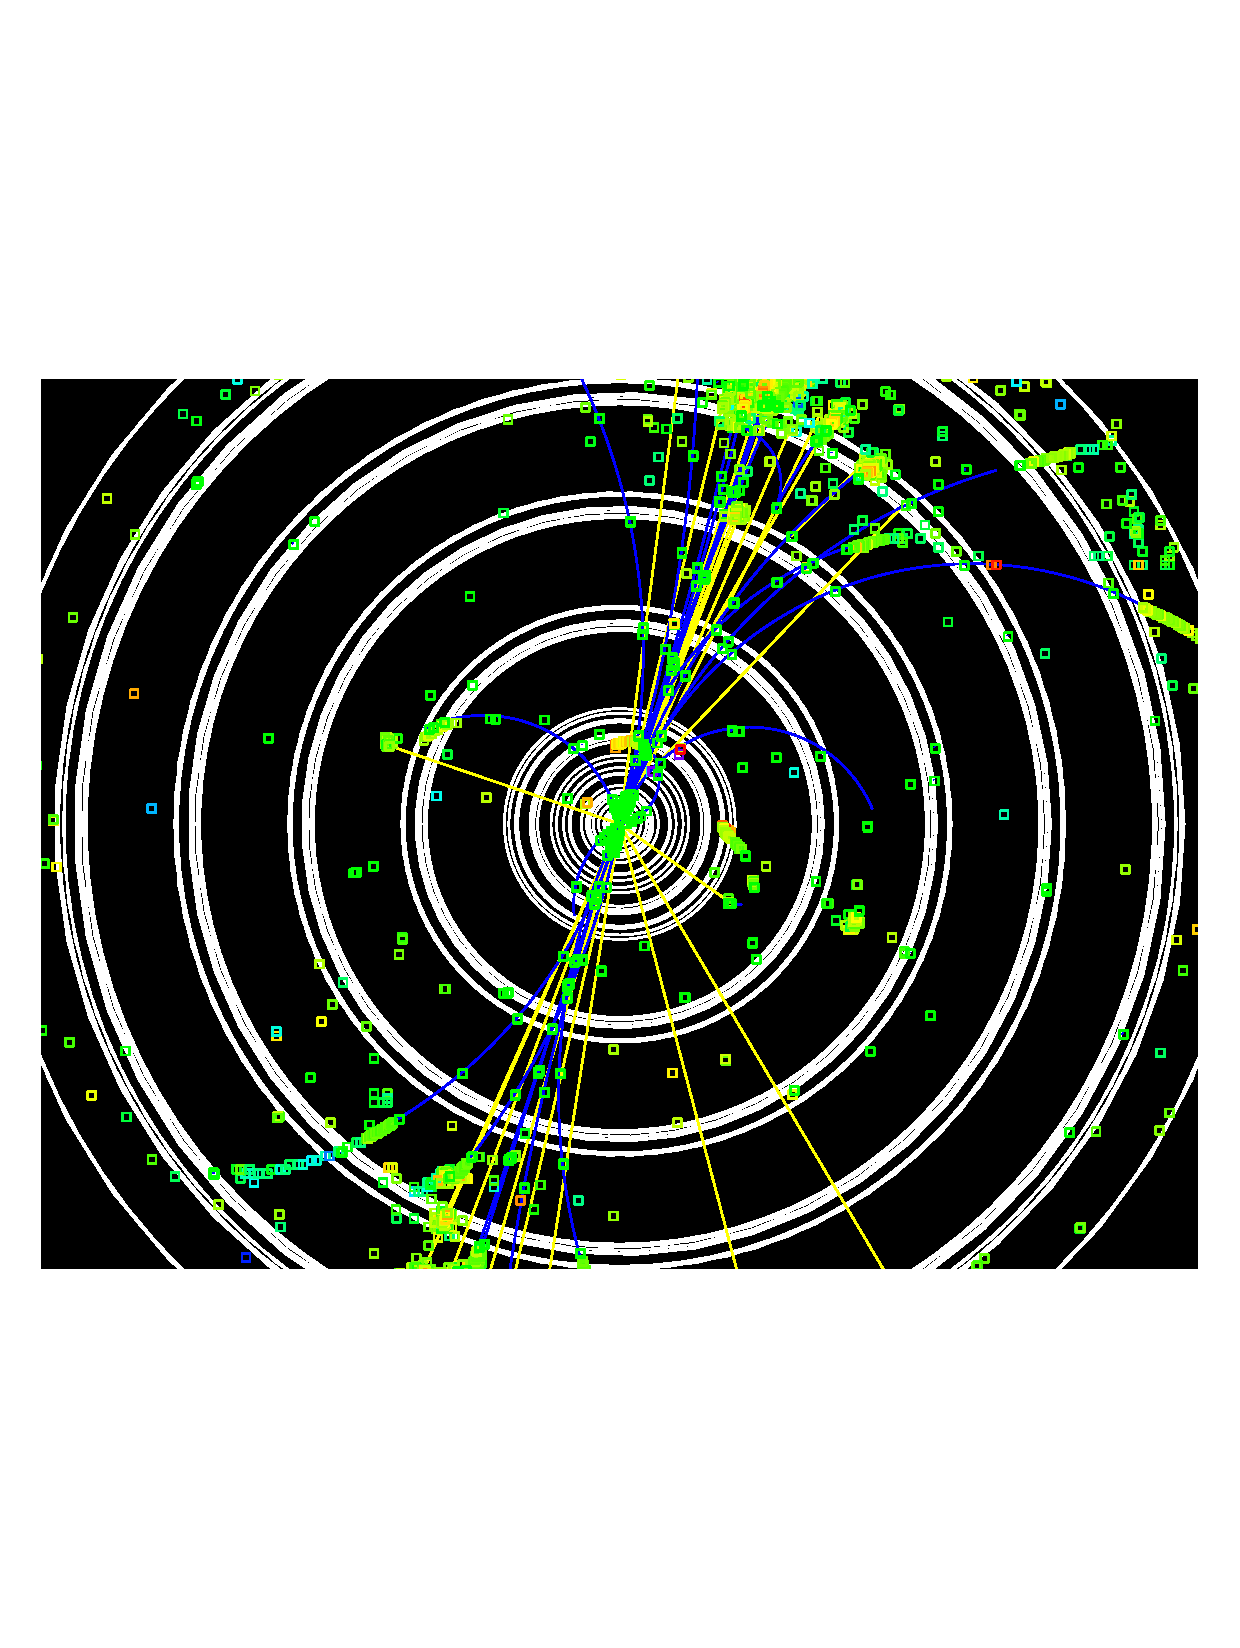
\includegraphics[scale=.5]{./Images/Wired_View_1.pdf}
	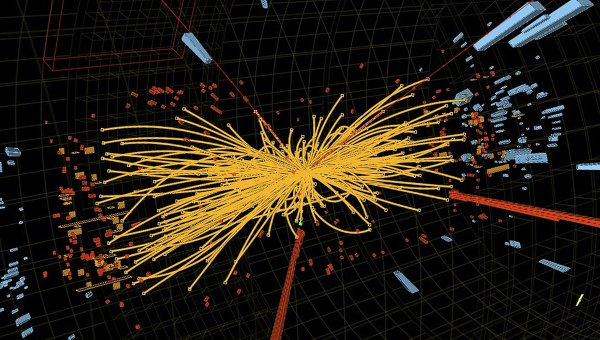
\includegraphics[width=.9\textwidth]{higgs}
	\vspace{\stretch{5}}
	
	\myTime
     %\end{flushright}
     \end{center}
  \end{addmargin}       
\end{titlepage}



%\begin{titlepage}
%{
%        \large  
%
%        \hfill
%
%        \vfill
%
%        \begingroup
%            \color{Maroon}\spacedallcaps{\myTitle} \\ \bigskip
%        \endgroup

%        \spacedlowsmallcaps{\myName}

%        \vfill

        %\includegraphics[width=6cm]{gfx/TFZsuperellipse_bw} \\ \medskip

        %\mySubtitle \\ \medskip   
        %\myDegree \\
        %\myDepartment \\                            
        %\myFaculty \\
        %\myUni \\ \bigskip

%\vfill
%}

%        \textsw{\myTime}
%\ -- \myVersion

%        \vfill                      

%    \end{center}  
 % \end{addmargin}       
%\end{titlepage}   





%*******************************************************
% Titlepage
%*******************************************************
%\begin{titlepage}
%\pdfbookmark{Titlepage}{Titlepage}
%\changetext{}{}{}{((\paperwidth  - \textwidth) / 2) - \oddsidemargin - \hoffset - 1in}{}
%\null\vfill
%\begin{center}
%\large
%\sffamily

%\bigskip

%{\Large\spacedlowsmallcaps{\myName}} \\

%\bigskip

%{\huge\spacedlowsmallcaps{\myTitle} \\
%}

%\bigskip
%{\large\spacedlowsmallcaps{\mySubTitle}} \\

    
%\vfill
%\vfill
%\vfill
%					{\normalsize
					
%        \myTime}
%\end{center}
%\end{titlepage}



\clearpage



%*******************************************************
% Titleback
%*******************************************************
\newpage
~\vfill
\thispagestyle{empty}


	       \ifx\myName\@empty\else
	          \noindent Copyright \copyright{} \the\year~\myName\\
                  All rights reserved.
	      \fi
%\noindent \textsc{Published by Publisher}\\ % Publisher

\noindent {\textsc{E-mail}:~\mail{alessandro.candolini@gmail.com}}\\

%%{\small \noindent{\spacedlowsmallcaps{E-mail}}: 
%%\mail{alessandro.candolini@gmail.com}}
%\noindent Licensed under the Creative Commons Attribution-NonCommercial 3.0 Unported License (the ``License''). You may not use this file except in compliance with the License. You may obtain a copy of the License at \url{http://creativecommons.org/licenses/by-nc/3.0}. Unless required by applicable law or agreed to in writing, software distributed under the License is distributed on an \textsc{``as is'' basis, without warranties or conditions of any kind}, either express or implied. See the License for the specific language governing permissions and limitations under the License.\\ % License information

\noindent \textit{First printing, September 2014} % Printing/edition date



%\thispagestyle{empty}

%\hfill

%\vfill

%\noindent\myName: \textit{\myTitle}
%\textcopyright\ \MakeTextLowercase{\myTime}.

%\medskip
%\medskip
%\noindent{\spacedlowsmallcaps{E-mail}}: \\
%\mail{alessandro.candolini@gmail.com}

%\vspace{1cm}
%%\hrule
%\bigskip

%%\noindent The titlepage reproduces an engraving of Maurits Cornelis Escher, titled \emph{Plane Filling with Birds} (the picture is obtained from \url{http://www.mcescher.com/}).



%*******************************************************
% Dedication
%*******************************************************
\cleardoublepage
\thispagestyle{empty}
\pdfbookmark[1]{Dedica}{Dedica}

\vspace*{3cm}

\selectlanguage{english}
\begin{quotation}
   \openquote 
  There is nothing more practical than a good theory.~\closequote
\begin{flushright}
    --- Kurt Lewin, 1945 
\end{flushright}
%\end{center}
\end{quotation}












%\input{FrontBackmatter/Sommario+Abstract}
%\input{FrontBackmatter/Pubblicazioni}
%% !TEX encoding = UTF-8
% !TEX TS-program = pdflatex
% !TEX root = ../Tesi.tex
% !TEX spellcheck = it-IT

%*******************************************************
% Ringraziamenti
%*******************************************************
\cleardoublepage
\phantomsection
\pdfbookmark{Ringraziamenti}{ringraziamenti}

\begin{flushright}{\slshape    
	Lorem ipsum dolor sit amet, consectetuer adipiscing elit. \\
	Ut purus elit, vestibulum ut, placerat ac, adipiscing vitae, felis. \\
	Curabitur dictum gravida mauris.} \\ \medskip
    --- Donald Ervin Knuth
\end{flushright}


\bigskip

\begingroup
\let\clearpage\relax
\let\cleardoublepage\relax
\let\cleardoublepage\relax

\chapter*{Ringraziamenti}

\lipsum[1]

\bigskip
 
\noindent\textit{\myLocation, \MakeTextLowercase{\myTime}}
\hfill L.~P.

\endgroup
\pagestyle{scrheadings} 
%*******************************************************
% Contents
%*******************************************************
\cleardoublepage
%\phantomsection
%\pdfbookmark{\contentsname}{tableofcontents}
\setcounter{tocdepth}{2}

\begingroup 
    \let\clearpage\relax
    \let\cleardoublepage\relax
    \let\cleardoublepage\relax
\tableofcontents
\endgroup
\markboth{\spacedlowsmallcaps{\contentsname}}{\spacedlowsmallcaps{\contentsname}} 

\cleardoublepage


%*******************************************************
% Prefazione 
%*******************************************************

\myChapter*{Preface}
\addtocontents{toc}{\protect\vspace{\beforebibskip}}
\addcontentsline{toc}{chapter}{\numberline{}\tocEntry{Preface}}
%\markboth{\spacedlowsmallcaps{Preface}}{\spacedlowsmallcaps{Preface}} 

%\adjustmtc
%\mtcaddchapter[\numberline{}\tocEntry{Preface}]

This preface and these notes are written from a physicist' perspective. 
This will ultimately drive the approach towards the subject and it will bias the selection of topics
presented here,
the examples discussed throughout this work, and the
level of mathematical rigour (higher than what is customary in several books of practical statistics) ,
leading to prioritize definitely what is likely to be of major relevance or more common for an
audiance of physicists, nevertheless trying to emphasize at the same time the impacts, implications 
and applications 
in contemporary information technology and big data community.

A through understanding of traditional and modern 
statistical inference (theory, methodologies, techniques, and algorithms) 
has always been playing quite a prominent  
role in the education and training of a scientist (in general) and of a
physicist (in particular), providing the framework and the tools to analyse
in a reliable and rigorous way 
the outcomes of
either actual experiments 
or virtual computer simulations,
in order to get insights, estimate parameters and their accuracy and precision, make comparisons between theory and
experiments, validate 
hypothesis tests, assess the validity of a theoretical model and its underlying
assumptions against experimental data, and make predictions. 

The need of a powerful background in statistics has probably become even more
demanding in recent years for practitioners in data analysis. 
The exponential growth of computing resources during the past few decades has made
the last decades increasingly data-intensive.
Beyond ``traditional methods (\eg, probabilitic modelling, linear and non-linear  regression theory,
confidence intervals, theory of estimators,  statistical significance,
hypothesis test, time series analysis, etc), new computer-intensive powerful
techniques has emerged in the last decades, including new progress in
Bayesian statistics, maximum entropy methods, computational statistics
(montecarlo methods, expectation-maximization algorithm,
hidden Markov models, resampling techniques such as the statistical bootstrap, etc), statistical learning 
(artificial neural
networks, support vector machines, $k$-means clustering, and
related topics in pattern recognition, etc), just
to mention few examples. 



In this respect, 
physics has always been a rich source of probabilistic models.
(statistical
mechanics, etc).
statistical mechanics (lattice spin models such as Potts models or spin glasses, ergodic theory), group
theoretical methods and concepts borrower from 
relativistic 
quantum field theory  and high energy particle physics provide valuable
insights  to better understand 
the mechanism behind these tools.

From a theoretical viewpoint,
is a beautiful and
fashinating field of research, 
sharing 
important connections with information theory, mathematics, 
artificial intelligence and robotics, physics (\eg, statistical
mechanics), etc. 
But the relevance of these methods is far from being just of theoretical
interest. 

From a practical viewpoint, statistical methods 
are undergoing a tremendus  development in recent years.
This is not only relevant for physics however.
playing an increasing widespread role  in modern information
technology and big data community, 
Warning about the misleading analysis and abuse of some statistical technique,
nevertheless 
helping in this way to popularize some cornerstone
machine learning techniques. 
while the size of data is posing challanging questions on how to efficiently
pro
and they 
have proved successful to approach data analysis in many
different areas, not only including physics, 
impacting 

Pervasiveness of distributed cloud-based clusters, crucially providing both the 
computational and the storage resources necessary for processing massive datasets;

The data-driven paradigm is emerging, the internet of things (IoT) is promising
an even more 
increasing  volume of 
data
to be digested in the upcoming years, 
pressing for successful strategies capable of 
processing at high rate (or even in real-time) massive distributed datasets. 

Mastering these topics requires a mix of knowledge, skills and experience to
succeed, together with high proficiency with related algorithms and their
implementation. 
Familiarity with algorithms
and ability to efficiently implement them 
is an essential part, 
and it can become even less trivial when the data requires distributed or
high-performance computing.


Two schools: frequentist and Bayesian.
Unfortunately, there is no general consensus among statisticians (and even
among physicists)

The aim of this notes is slightly ambitious.
First, thoroughly  discuss at  graduate level the 
 theoretical underpinnings of traditional and modern statistical tools and
 their 
 mathematical foundations, establishing the main results and developing theoretical
 tools.
 I firmly believe that 
 it is not possible to perform a reliable data analysis without a solid
 knowledge of the theory behind those tools: theory is essential to understand and control the
range of  validity of a given method, to understand how to inspect the results,
and to highlight artifacts (which are always
present), and in case to develop custum solutions for the problem at hand. 
In the second part, we will discuss concrete examples, together with actual implementation of algorithms to handle data
analysis in real examples. 
This will help to illustrate pitfalls, best practises, implementation
strategies, libraries and platforms, etc


		\vskip2ex

\mySignature{\myLocation, \myTime}{\Large{\calligra\myName}}

\cleardoublepage
% *****************************************************************************
% Materiale principale
% *****************************************************************************
\cleardoublepage
\pagenumbering{arabic}
\cleardoublepage
%\ctparttext{}
\ctparttext{This part deals with the theory of probability.
   The rigorous definition of probability  is given, according to Kolmogorov.
   Then, its properties are derived, a number of recurrent common probability
   distributions are introduced together with tools to handle them (among them
   are: probability distributions, characteristic functions, moments, etc) and
   finally few important limit theorems are established.  The theory of
   probability is important by its own and it is at the same time the natural
   prerequisite for statistics.}
\part{Probability}
%
%*******************************************************
% Chapter 1
%*******************************************************

\myChapter{Introduction}

This chapter gives an overview of the subject and discuss 
the roadmap of the next chapters.

\section{Top 10 algorithms in data mining}
In an effort to identify some of the most influential algorithms in data
mining, 
the IEEE International Conference on Data Mining
identified the following top 10 algorithms:
\footcite[See][]{Wu.Kumar.ea:2007}
\begin{itemize}
   \item C4.5 (decision trees)
   \item The $k$-means algorith;
   \item Support vector machines (SVM);
   \item The Apriori algorithm;
   \item The EM algorithm;
   \item PageRank;
   \item AdaBoost;
   \item $k$-Nearest Neighbor classification;
   \item Na\"{\i}ve Bayes;
   \item CART.
\end{itemize}

\section{Goals}

These notes are aimed at developing a throughly understanding of the Top 10
algorithms un data mining, from both theoretical and practical perspective.

It is intrinsically cross-field subject, requiring knowledge from different
fields (statistics, mathematics, etc)
Moreover, it requires to grasp computer science at several different scales.
Require widespread knowledge  of several different fields.
\begin{itemize}
\item Programming languages: different companies uses different programming
   languages and/or software tools; some languages are useful because they
   allow less developing time, some other are more suitable for high
   performance computing, some other have powerful and highly maintened
   libraries, some other are the ones employed in large scale distributed
   platforms. So you need to somewhat familiar and confident with several
   programming language, to choose the one most suitable for your task or to
   integrate 
\item Feature extraction
\item Data cleaning
\item Knowledge of non trivial statistics  needed in the background
\item Mathematics involved in these algorithms is not trivial, but you need a
   deep knowledge of the algorithms in order to understand 1) where they are
   epected to be the best option to approach the problem, 2) how to improve the
   algorithm for the problem at hand, 3) to gain better understanding of the
   results of the algorithm (to catch artifacts, etc)
\item Database
\item Visualization
\item Debuggin
\item Intuition
\end{itemize}

There is (and there can be) no single source covering well all these aspects of
machine learning. Of course, there would be not enough room in a single volume to explore
in details all these things. However, here we will try to procee d in a way to
offer at the reader 1) knowledge of the key algorithms, 2) implementing those
algorithms in full details in some programming language to attack simple
problems, 3) and try to make a full analysis of real problems to show some
examples, trying to
fill the gap between theory and practice. It goes without saying that some
choices will be a matter of taste. For example, we will need to choose a
programming language. We will discuss to some extend pro and cons of different
programming languages.

Out approach will be
\begin{itemize}
   \item Python: best tool to quick explore the data, data visualization etc
   \item \cpp{} to develop heavy programs
\end{itemize}

We will also give a quick account of some other tools, for example
\begin{itemize}
   \item TMVA: Root Cern machine learning framework used in High energy physics
   \item Tools in R
\end{itemize}
but we will not use them extensively in the applications.

Regarding the use of Java, this is mostly related to Hadoop and related
Map-Reduced implementations. 



%\myChapter{TVMA}
%\myChapter{HDF5}
%\myChapter{MLPACK}



%*******************************************************
% Chapter 1
%*******************************************************

\myChapter{Kolmogorov axioms}

\begin{refsection}

   Rigorous foundation of mathematical probability is provided by
   Kolmogorov's measure-theoretical approach%
   \footcite{Kolmogorov:1956}.
   In this framework, the mathematical notion of probability is defined in an abstract way by 
   all and only the rules that any probability must fulfill.
   Among the strenghts of this approach is the fact that it 
   completely \emph{decouples} the definition of probability from empirical
   notions and conceptual interpretations. 
   Kolmogorov's axioms provides the rules of the game, allowing to establish
   properties of probability and ways to manipulate mathematical
   probabilities on a general ground, without relying on a specific way to
   assign values to a probability. 
   In order to apply the theory to study a particular situation, one should supply the
   framework with a concrete ``probabilistic model''
   (\ie, she/he should assign a probability)
   suitable for the example at hand; the choice and the construction of the
   probabilistic model is an empirical ``input'' which should be provided
   externally to
   the Kolmogorov framework.

   It is worth mentioning that Kolmogorov's approach to mathematical
   probability is not free from criticism. 
   An introductory review of approaches to probability and their conceptual
   interpretation 
   are  briefly sketched
   in \cref{sec:other_probability}.

   \begin{figure}
\centering
\subfloat[][]{%
   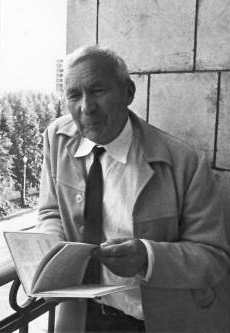
\includegraphics[width=.45\columnwidth]{Kolmogorov}%
   \label{fig:kolmogorov}%
}
\quad
\subfloat[][]{%
   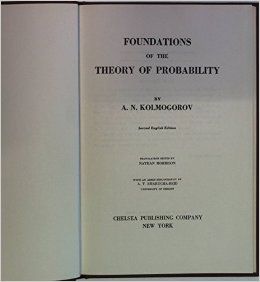
\includegraphics[width=.45\columnwidth]{Kolmogorov_book}%
   \label{fig:kolmogorov_book}%
}
\caption{%
   \protect\subref{fig:kolmogorov} Russian mathematician Andrey Nikolaevich Kolmogorov
   (1903--1987). Source: Wikipedia.
   \protect\subref{fig:kolmogorov_book} Title page of english edition of
   Kolmogorov's \emph{Foundations of the theory of probability}.
}
\end{figure}

\section{Crash course in abstract measure theory}

Kolmogorov axioms are rooted in abstract measure theory.
Since this is a fairly advanced topic in mathematics, we give here a brief
account of the very basic of this subject in order the Reader to be accustomed
to it at least to some extend%
\footcite[For a more comprehensive treatment and its application to rigorous
probability, refer to, \eg,
][]{Kolmogorov:1956,Billingsley:1995,Rosenthal:2006}.

Roughly speaking, the ultimate goal is that of  appending some reasonable
notion of ``measure'' to the subsets of a given non-empty set (the precise mathematical definition of
measure coming 
soon). Troubles eventually arises however when dealing with sets having
uncountable many items if one tries to apply the notion of measure naively to
all subsets of such sets. The famous Banach-Tarsky paradox
is the  prototype of the  kind of difficulties one encounters.

\begin{approfondimento}
For those who are not familiar, a discussion of the Banach-Tarsky
paradox can be found, \eg, in \cite{Stromberg:1979}
and references therein. 
Proof of Banach-Tarsky paradox is highly non-trivial and it relieas technically on  the axiom of
choice. 
Nevertheless, the statement of the theorem itself is paradigmatic on the kind
of difficulties one meets when dealing with uncountable sets.
\end{approfondimento}


   To overcome the aforementioned difficulties when trying to ``measure'' a subset of a set, at a techical level one resorts to constrain
the definition of 
``measure'' over suitable collections of subsets called $\sigma$-algebras. 

Let 
$\Omega$ be any set.
Hereafter, $2^{\Omega}$ will denote the ``power set'' of $\Omega$, \ie, 
the set of 
   all and only the subsets of
   $\Omega$. 
   In
   axiomatic set theory, the existence of $2^{\Omega}$ for every set $\Omega$
   is a postulate%
   \footnote{The axiom of power set is one of the Zermelo-Fraenkel axioms. It allows a simple definition of the Cartesian product of two sets, which in turn allows to define the notion of application between sets.}.


\begin{definition}[$\sigma$-algebra]
	Let $\Omega$ be any \emph{non-empty} set and 
   $\Sigma \subseteq 2^{\Omega}$ any arbitrary subset of the power set.
	$\Sigma$ is called 
	a $\sigma$-algebra over
   $\Omega$ if 
   \begin{enumerate} [label=(\alph*)]
      \item\label{item:sigma1} $\Omega \in \Sigma$;
      \item\label{item:sigma2} for every $A \subseteq \Omega$, if $A \in \Sigma$ then $
	 \complement{A}{\Omega}\in \Sigma$;
      \item\label{item:sigma3}for every sequence
	 $\fullfunction{(A_{n})_{n\in\N}}{\N}{\Sigma}$ of subsets of $\Omega$
	 belonging to $\Sigma$,
	 $\bigcup_{n\in\N} A_{n} \in \Sigma$.
   \end{enumerate}
\end{definition}

In words:
\ref{item:sigma1} implies that any $\sigma$-algebra is \emph{non-empty}.
\ref{item:sigma2} means a $\sigma$-algebra is closed under the
complementation: if an arbitrary subset $A$ belongs to $\Sigma$ then also its complementary $\complement{A}{\Omega}$ belogs to it. 
\ref{item:sigma3}  means that the $\sigma$-algebra is closed under
\emph{countable}
unions. 
This latter assumption might look rather technical at this level.
Why not just restrict ourselves to the union of a \emph{finite} (instead of countably infinite) number of subsets?
As we shall see later, \ref{item:sigma3} 
allows 
to handle convergence theorems, to take limits of sequences of subsets,  etc. 

   \begin{remark}
   The empty set $\varnothing$ also belongs to any $\Sigma$-algebra. 
	   Proof: 
by 
\ref{item:sigma1} $\Omega$ belongs to $\Sigma$;
	   \ref{item:sigma2}, its complement $\complement{\Omega}{\Omega} = \varnothing$ must belong to 
$\Sigma$. 
\end{remark}

\begin{example}
	Given any set $\Omega$, 
   the subset $\Set{\Omega, \varnothing}\subseteq2^{\Omega}$ consisting only of the empty set
   $\varnothing$ and the set $\Omega$ itself is a $\sigma$-algebra over $\Omega$; it is called
   the ``minimal''
or ``trivial'' $\sigma$-algebra over $\Omega$.
\end{example}
\begin{example}
   Let $\Omega$ be a non-empty set having a non-trivial subset
   $A\subseteq\Omega$.
   The subset $\Set{\Omega, A, \complement{A}{\Omega},
      \varnothing}\subseteq2^{\Omega}$ 
   is a $\sigma$-algebra over $\Omega$.
\end{example}

\begin{example}
   The power set $2^{\Omega}$ of a set $\Omega$ is a $\sigma$-algebra over
   $\Omega$, called
   the ``discrete'' $\sigma$-algebra.
\end{example}

A set endowed with a sigma algebra is called a ``measurable space''; the reason
for this name is that it is always possible to define a ``measure'' on it.
More formally, we have the following definition.

\begin{definition}[Measurable space]
   An ordered pair $(\Omega, \Sigma)$ where $\Omega$ is an arbitrary set and
   $\Sigma$ is any $\sigma$-algebra over $\Omega$ is  called 
   a ``measurable space''.
\end{definition}

\begin{lemma}
   Let $(\Omega, \Sigma)$ be any measurable space.
   Then, for every sequence $\fullfunction{(A_{n})_{n\in\N}}{\N}{\Sigma}$ of
   elements in the $\sigma$-algebra $\Sigma$, we have
   \begin{dmath*}
      \bigcap_{n\in\N} A_{n} \in \Sigma
   \end{dmath*},
   \ie, any $\sigma$-algebra is also closed with respect to countable
   intersection.
\end{lemma}
\begin{proof}
   DeMorgan rules + induction.
\end{proof}


   \section{Set theory definition of probability}
   

   Dice: \drawdie{1} 

   \section{First properties of probability}

   \begin{figure}
      \centering
      \begin{venndiagram2sets}[overlap=-1cm,labelNotAB={$\Omega$}]
	 \fillACapB
      \end{venndiagram2sets}
      \caption{Union}
   \end{figure}


   \section{Borel-Cantelli lemmas}

   \section{Discrete probability space}


   Before continuing with the discussion of probability measures in
   their full generality, it is helpful to consider the simpler case where the
   sample
   space $\Omega$ is finite or countable.

   \subsection{Dices}

   \subsection{Urns}

   \subsection{Coupon collector problem}
   
   \section{Bertrand paradox}

   \section{Conditional probabilities and independent events}


   \begin{definition}[Conditional probability]
      \label{def:conditional_probability}
      Let $(\Omega, \Sigma, \P{\cdot})$ be a probability space and $A,B\in
      \Sigma$ such that $\P{B} > 0$. The ``conditional probability of $A$ given
      $B$ is defined as 
      \begin{dmath}
	 \P{A\given B}  \coloneqq \frac{\P{A \cap B }}{\P{B}}
      \end{dmath}.
   \end{definition}

   \begin{remark} 
      The definition makes sense since $A,B \in \Sigma$ implies $A\cap B\in
      \Sigma$ (being $\Sigma$ a $\sigma$-algebra).
      The condition $\P{B} > 0$ is required otherwise the denominator on the
      right-hand side would vanish.
   \end{remark}

 Set interpretation of 
      \cref{def:conditional_probability}:
      $\P{A\given B}$ can be visualized as if we were restricting the sample
      space to the subset $B$ alone. The logic
      behind this equation is that if the outcomes are restricted to B, this
      set serves as the new sample space.

   \section{Bayes' theorem}


%   \begin{advanced}
%      \section{Bayes theorem made simple using LEGO bricks}
%   \end{advanced}
%
%   This section is inspired by a online blog from Will Curt%
%   \footcite{Onl-curt:2015}.

   \section{A panorama of approaches to probability}
   \label{sec:other_probability}


   No attempt will be make at discussing the deep philosophical  implications
of applying the Kolmogorov's framework.

A review is done by \cite[][\S~1]{Feller:1966}.
See also \cite{Cox:1946}.
For a review of Cox, see \cite{Van-Horn:2003}.
See also \cite{Jaynes.Bretthorst:2003}.


   \section{What's the use of all this?}

   The usefulness of abstract measure theory extends far beyond the Kolmogorov's
   foundation of mathematical probability, and find broad applications 
   in other areas of applied mathematics and physics as well%
   \footcite[Just to make one example, refer to, \eg, ][\S~13, for an application of measure-theoretical
   concepts to classical ergodic theory, chaotic dynamical systems and
   classical equilibrium statistical mechanics.]{Fasano.Marmi:2006}.


   From a practical viewpoint, it would have been possible to develop a more
   intuitive theory of probability 
    relying on 
   the more familiar concepts of probability distributions and densities, to be
   developed in
   the next chapter%
   \footcite[An example of this approch is offered by the first chapter
   of][]{Van-Kampen:2007};
   these tools are very useful to study the simplest cases. 
   Nevertheless, such approach would have been less general and 
   inadeguate to formulate rigorously some limit theorems. 
   Using sets rather than
   distributions to define the probability
   allows for a more general and powerful treatment, even though it leads to
   some mathematically-intensive formulation at the beginning.

   Kolmogorov's axioms provide a theoretical framework to define
   probability in a abstract way, emphasizing its mathematical ``structure''
   and properties,
   regardless on the specific  empiric 
   applications. 
   In order to 
   to apply this framework to real-life applications, one must first build a suitable
   probabilistic model (\ie, provide a specific choice of
   the probability measure) to this framework. 
   Statistics (to be discussed in later chapters) is concerned with inferring
   the ``most appropriate'' (a least to some extend) probabilistic model (out of some range of models) from
   inspection of the available empirical data. 
   The basic properties of probability established on this chapter will be use
   throughout all the following chapters. 

   The importance of Bayes theorem cannot be understimated: 
   beyond being of major importance by its own, it plays a decisive 
   role in the foundation of Bayesian inference (more on this in later chapters). 


\printbibliography[heading=subbibliography]
\end{refsection}


%*******************************************************
% Chapter 1
%*******************************************************

\myChapter{Random variables}
\label{chap:random_variables}

\begin{refsection}

   Discrete and continuous, univariate and multivariate real random variables are
   discussed, together with a bunch of practical tools helping to handle with
   them, specifically: probability
   density function, cumulative distribution function, moments
   (\ie, mean, variance, skewness, kurtosis, etc).
   All of this provides a more concrete, visualizable approach to probability
   built on top of the
   construction of the previous chapter by means of probability measures; it should be stressed however
   that the probability measures provides a more general framework. 
   This chapter also covers functions of random variables, change of variables
   (\ie, what physicists are accustomed to call ``propagation of errors''), etc.
   Generating functions --- another useful tool to deal with probability
   distributions --- are postponed to \cref{chapt:generating_functions}: an
   entire chapter is devoted to them 
   since their theory and their application deserve special attention. 
   More general  random variables (\eg, matrix-valued random variables)
   although useful are not presented here (see however
   \cref{chap:random_matrices}, which is 
   devoted to a brief account of random matrix
   theory).

   \section{Definitions and basic properties}

      Let 
      \begin{inparaenum}[(a)]
      \item $(\Omega, \Sigma, \P{\cdot})$ be any probability space;
	 \item $(E, \epsilon)$ be any measure space;
	 \item $\fullfunction{X}{\Sigma}{E}$ be any (measurable) function from
	    $\Sigma$ to $E$.
      \end{inparaenum}
      In this context: $\Omega$ is called the ``sample space'', $E$ is called ``state space'',
      $X$ is called a ``random variable'', ``aleatory variable'' or ``stochastic variable''.

      Whenever the range $X(\Sigma) \subseteq E$ of $X$ has finite or countably
      infinite cardinality, the
      random variable $X$ is called a ``discrete'' random variable.
      When the range of $X$ is uncountably infinite instead, $X$ is called a
      ``continous'' random variable. 

      In this chapter, we will be mainly interested in the  case of \emph{real}-valued
      (discrete or continuous) univariate (\ie, $E \subset \R$) or multivariate
      (\ie, $E\subseteq \R^{N}$, $N\in\N$, $N\geq 2$) random variables (the
      Borel algebra being the underlying $\sigma$-algebra in the state space).
      For such case, it makes sense and it proves useful to introduce the
      important concepts of moments, distribution functions, etc. (Those definitions are
      slightly different whether the random variable is discrete or continuous
      and univariate or multivariate,
      as we will see shortly.)
      However, the definition of random variables applies to more general
      settings; for example, in \cref{chap:random_matrices} the case where $E$
      is a suitable space  of matrices 
      will be taken into account.
      Other scenarios are also possible (\eg, random graphs, etc) some being
      relevant for statistical mechanics, machine learning, etc (see later chapters).


   It is worth notice that random variables take value over the set $E$,
   nevertheless $E$ is not the probability space itself; the random variable
   instead is defined as a mapping defined over a suitable $\sigma$-algebra
   of an underlying probability
   space $\Omega$ and targetting the (measure) state space $E$. 

   What is the benefit of having defined a random variable as a mapping from a
   probability space to the state space $E$ instead of having $E$ itself
   equipped with a suitable probability
   measure?

   \section{Probability distribution}

   In most applications, the underlying probability space defining a random
   variable remains hidden.
   Instead, a ``distribution function'' is introduced which 



   \subsection{Univariate discrete random  variable}
   \subsection{Univariate continuous random variable}
   \subsection{Multivariate discrete random variable}
   \subsection{Multivariate continuous random variable}

   \section{Moments of a distribution}
   \section{Transformations of random variables}
   \section{Buffon's needle}

   \section{What's  the use of all this?}

\printbibliography[heading=subbibliography]
\end{refsection}


%*******************************************************
% Chapter 1
%*******************************************************

\myChapter{Catalog of probability distributions}

The tools developed in \cref{chap:random_variables} are applied to a list of
important discrete and continuous, univariate and multivariate probability distributions. 
These distributions are the building blocks of several probabilistic models and
are relevant for later applications in statistics, so it is worth browsing
through all the details and calculations. 

\section{Discrete distributions}

\subsection{Bernoulli distribution}
   \label{sec:bernoulli_distribution}
\subsection{Binomial distribution}
   \label{sec:binomial_distribution}
\subsection{Poisson distribution}
   \label{sec:poisson_distribution}
\subsection{Hypergeometric distribution}
   \label{sec:hypergeometric_distribution}
\subsection{Multinomial distribution}
   \label{sec:multinomial_distribution}


\section{Continuous distribution}

\subsection{Uniform distribution}
   \label{sec:uniform_distribution}
\subsection{Exponential distribution}
   \label{sec:exponential_distribution}
\subsection{Cauchy distribution}
   \label{sec:cauchy_distribution}
\subsection{Univariate normal distribution}
   \label{sec:normal_distribution}
\subsection{Multivariate normal distribution}
   \label{sec:multinormal_distribution}
\subsection{Chi-square distribution}
   \label{sec:chisquare_distribution}
\subsection{$t$-student distribution}
   \label{sec:tstudent_distribution}
\subsection{Gamma distribution}
   \label{sec:gamma_distribution}
\subsection{Beta distribution}
   \label{sec:beta_distribution}
\subsection{Weibull distribution}
   \label{sec:weibull_distribution}

\section{What's the use of all this?}


%*******************************************************
% Chapter 1
%*******************************************************

\myChapter{Generating functions}
\label{chapt:generating_functions}
\begin{refsection}
Generating functions are a overwealming  weapon to attack irresistable problems
which fail a 
more straightforward approach. 
In this section we will introduce the notion of generating function, we will
establish the relevant properties and we apply the technique of generating
functions to few prototypical examples, in particular involving the famous
Fibonacci numbers and the integer partitions. 
In later chapters, the technique of generating functions will prove useful for
example to deal with Galton-Walton problem.
In statistical mechanics, the generating function approach is related to the
grancanonical partition function.
The main source for this chapter is \cite{Wilf:1994}.


   \section{Fibonacci numbers as a prototype}
   \label{sec:fibonacci}
   The  sequence $(\Fibonacci{n})_{n\in\N}$  of Fibonacci numbers can be defined in a number of equivalent ways and
historically made its first appearance in connection with a combinatorial
model (the rabbit's population model described below).
One definition is the following: the sequence $(\Fibonacci{n})_{n\in\N}$ of
Fibonacci numbers is defined as 
the \emph{unique} solution of 
\begin{dmath}[label={Fn}]
   F_{n+2} = F_{n} + F_{n+1} \condition*{n\in\N}
\end{dmath}
satisfying the initial conditions
\begin{dseries}
   \begin{math}
      F_{0} = 1
   \end{math},
   \begin{math}
      F_{1} = 1
   \end{math}.
\end{dseries}
\Cref{eq:Fn} is a second-order homogeneous linear recursive equation with
constant coefficients, the general theory of such equations ensure that there
exists one and only one solution of it satisfying the initial valued problem.






   \section{Definition and properties of generating functions}

   \section{Solution of Fibonacci recurrence using generating functions}

   

\printbibliography[heading=subbibliography]

\end{refsection}


%*******************************************************
% Chapter 1
%*******************************************************

\myChapter{Limit theorems}

\begin{refsection}

   \section{Inequalities}

   

\printbibliography[heading=subbibliography]

\end{refsection}

\ctparttext{The material in this part might  appear to be slightly departing from the
   core topics of these notes, namely 
   statistics, however much of the material is relevant for stochastic
   modelling. 
}
\part{Additional Topics in Probability}

%*******************************************************
% Chapter 1
%*******************************************************

\myChapter{Stochastic processes}

\begin{refsection}



   

\printbibliography[heading=subbibliography]

\end{refsection}


%*******************************************************
% Chapter 1
%*******************************************************

\myChapter{Markov processes}

\begin{refsection}

   An important class of stochastic processes is provided by the so-called
   Markov processes. 
   Markov processes are ubiquitous.
   They are a relevant ingredient for  
   stochastic modelling and they provide the theoretical basis of important
   statistical and coomputational techniques, ranging
from Markov-chain Montecarlo to hidden Markov models, discussed in later
parts.
   This chapter serves as an introduction to
   their definitions and first properties, and illustrates few beginning examples. The
   material is indispensable also for later chapters. 

   The following stochastic processes \emph{need not} to be Markovian.
   They can be Markovian in some special cases but they do not need to be
   Markovian in general 
   and allow for special treatment.
   For example, the simple  random walk is Markovian; the self-avoiding random
   walk is a prototypical example of a \emph{non}-Markovian process.
   For this reason, these processes will be discuss in later chapters:
   \begin{itemize}
      \item random walks;
      \item branching processes.
   \end{itemize}
   As prototypes of Markov processes we will discuss:
   \begin{itemize}
      \item Erenfest urn;
      \item \google{} \pagerank{} ranking algorithm;
      \item Applications of Markov processes to shopping;
      \item Solution of the coupon problem via Markov chains.
   \end{itemize}
   In later chapters, we will discuss modern topics like
   \begin{itemize}
      \item Markov chain Montecarlo and Metropolis-Hasting algorithm in
	 computational statistical mechanics and computational Bayesian
	 inference;
      \item Hidden Markov models.
      \end{itemize}
      Both heavily relies on Markov processes.
      The stochastic calculus and the chapter on stochastic differential
      equation makes use of Wigner integrals which are based on Markov
      processes.
	 

      \begin{figure}
	 \centering
	 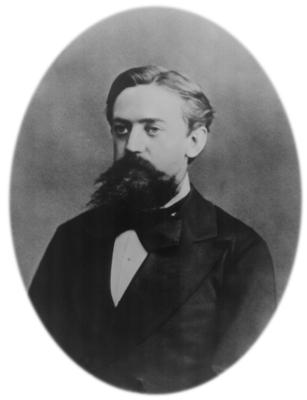
\includegraphics[width=.40\textwidth]{AAMarkov}
	 \caption{Russian mathematician Andrei Andreyevich Markov
	    (1856--1922), the father of Markov processes.}
      \end{figure}

      \section{Markov property}

      Intuitively speaking,
      Markov processes are \emph{memoryless}: the probability of evolving from
      the current state to the 
      next one does not depend on the previous history of the process.
      The exact mathematical implementation of this concept can look a bit
      technical for Markov processes defined on continuous state spaces and
      continuous index space, but for finite settings it should be easier to
      grasp.
      For this reason, we first define the general notion for arbitrary
      (continuous) processes but later we will mainly focus on the finite
      setting, where Markov processes are more often called ``Markov chains''.
      Markov chains  will be enough for most of our purposes.
      General Markov processes occur however in many situations (Brownian
      motion, Markovian evolution of open quantum systems, etc); for this
      reason, we give the general definitions.


      \section{Ergodicity}
      \section{Stationary  distribution}

      \section{Remarks on non-Markovian
	 processes}
      \footcite{Van-Kampen:1998}

      

      

      \section{The coupon problem revisited}   
      \section{Erenfest urn}
      \section{Shopping model}
      \section{\google{} \pagerank{} algorithm}
In the early days of web search engine, 


Web search engines usually work in this way:
\begin{inparaenum}[(a)]
   \item Web Crawling 
   \item Indexing 
   \item Ranking 
\end{inparaenum}
First of all, an automated Web crawler retrieves and stores information from the HTML
markup of several many web pages. 
Data is analyzed and stored in a index database for use in later queries. 
Finally, when a query is performed by the user, the list of matching results
needs to be sorted by some criteria (ranking).


The \pagerank{} algorithm was 
has a lot of interesting mathematics behind it.  
In this note we will use the \pagerank{} algorithm a  a prototypical model and
as a pathfinder to explore and to illustrate some interesting mathematics behind
it.
We will give also a toy implementation of the algorithm to start playing with
it so to discover some of its features. 



\printbibliography[heading=subbibliography]
\end{refsection}


%*******************************************************
% Chapter 1
%*******************************************************

\myChapter{Poisson processes}

\begin{refsection}

   Poisson processes and their characterization is presented.


   \begin{advanced}
   \section{Lorentz classical model of elettrical conductivity in metals}
\end{advanced}

   \section{What's the use of all this?}   


\printbibliography[heading=subbibliography]
\end{refsection}


%*******************************************************
% Chapter 1
%*******************************************************

\myChapter{Random walks}

\begin{refsection}



   


\printbibliography[heading=subbibliography]
\end{refsection}


%*******************************************************
% Chapter 1
%*******************************************************

\myChapter{Branching processes}

\begin{refsection}

   For a superb account of branching processes, see \textcite{Harris:2002}.

   

\printbibliography[heading=subbibliography]

\end{refsection}


%*******************************************************
% Chapter 1
%*******************************************************

\myChapter{Glimpse at random matrix theory}
\label{chap:random_matrices}
\begin{refsection}



   


\printbibliography[heading=subbibliography]
\end{refsection}


%*******************************************************
% Chapter 1
%*******************************************************

\myChapter{It\^{o} Stochastic differential equations}

\begin{refsection}



   


\printbibliography[heading=subbibliography]
\end{refsection}

\cleardoublepage

\ctparttext{After introducing the basis of descriptive statistics, the core of
   frequentist and Bayesian inference are throughly studied.}
\part{Statistical inference}
\ctparttext{Machine learning techniques have been providing state-of-art
   performance in the analysis of massive datasets (even though some analysis
   at a rather heuristic level). This part deals with a rather introdoctory
   overview of some key  algorithms rooted in 
   machine learning and their statistical meaning.}
\part{Glimpse at statistical learning}

%*******************************************************
% Chapter 1
%*******************************************************

\myChapter{A panorama of machine learning techniques}
\label{chap:panorama}
\begin{refsection}

   

   The main source of material for this part is provided by:
   \begin{itemize}
      \item \textcite{Hastie.Tibshirani.ea:2009}
      \item \textcite{Bishop:2006}
   \end{itemize}

   \section{What's the use of all this?}
   


\printbibliography[heading=subbibliography]
\end{refsection}


%*******************************************************
% Chapter 1
%*******************************************************

\myChapter{Artificial neural networks}
\label{chap:nn}
\begin{refsection}


   \section{Models of electrical conductivity in neurons}

   \section{Perceptron}

   \section{Feed-forward neural networks and backpropagation algorithm}

   \section{Kohonen neural networks}

   \section{Associative memories}


   \section{What's the use of all this?}
   


\printbibliography[heading=subbibliography]
\end{refsection}


%*******************************************************
% Chapter 1
%*******************************************************

\myChapter{Support vector machines}
\label{chap:svm}
\begin{refsection}


   \section{What's the use of all this?}
   


\printbibliography[heading=subbibliography]
\end{refsection}


%*******************************************************
% Chapter 1
%*******************************************************

\myChapter{Glimpse at deep learning}

\begin{refsection}



   

\printbibliography[heading=subbibliography]

\end{refsection}

\ctparttext{A number of modern additional topics in statistics is covered, in
   particular modern 
   computational tools (expectation-maximization algorithm, hidden-markov
   models).}
\part{Advanced material and applications}

%*******************************************************
% Chapter 1
%*******************************************************

\myChapter{Kalman  filtering}
\label{chap:kalman}
\begin{refsection}

   


   \section{What's the use of all this?}
   


\printbibliography[heading=subbibliography]
\end{refsection}


%*******************************************************
% Chapter 1
%*******************************************************

\myChapter{Maximum entropy principle}
\label{chap:me}
\begin{refsection}


   \section{What's the use of all this?}
   


\printbibliography[heading=subbibliography]
\end{refsection}


%*******************************************************
% Chapter 1
%*******************************************************

\myChapter{Expectation-maximization algorithm}
\label{chap:em}
\begin{refsection}


   \section{What's the use of all this?}
   


\printbibliography[heading=subbibliography]
\end{refsection}


%*******************************************************
% Chapter 1
%*******************************************************

\myChapter{Hidden Markov Models}
\label{chap:hidden}
\begin{refsection}


   \section{What's the use of all this?}
   


\printbibliography[heading=subbibliography]
\end{refsection}


%*******************************************************
% Chapter 1
%*******************************************************

\myChapter{Potts models and spin glasses for image restoration}
\label{chap:potts}
\begin{refsection}


   \section{What's the use of all this?}
   


\printbibliography[heading=subbibliography]
\end{refsection}


%*******************************************************
% Chapter 1
%*******************************************************

\myChapter{Unfolding}
\label{chap:unfolding}
\begin{refsection}

   


   \section{What's the use of all this?}
   


\printbibliography[heading=subbibliography]
\end{refsection}

%\ctparttext{We throughly discuss the theory behind the most}
\part{Appendix}
\appendix

%*******************************************************
% Chapter 1
%*******************************************************

\myChapter{Rudiments of combinatorial analysis}

\begin{refsection}

Combinatorics is a branch of discrete mathematics mainly concerned with existence,
enumeration, classification and optimization of arrangements of
elements  of a given set according to 
prescribed rules, providing powerful tools to count, manage and establish
properties of these
arrangements. 
A review of the very basic  of the subject is mandatory here, since 
even the simplest exercises in probability (in the context of finite sample spaces having equally likely outcomes)
naturally demand for such tools to count in a smart way the number of certain
configurations in the sample space. 
(In fact, from an historical perspective, combinatorics was strongly motivated
by applications in 
probability.)
Much of the material presented here should be already well-known to a broad audience from
undergraduate (or maybe even high-school) courses, nevertheless we collect here
few important techniques  in combinatorial calculus which were used throughout the notes. 
Combinatorial problems can
quickly evolve 
from straightfoward to highly non-trivial and intractable ones and can make
their appearence in unexpected contexts: the final sections are devoted to few
more advanced topics maybe not directly related to probability aimed at
providing a 
flavor of what the whole combinatorics is all about, in order the Reader to acquire a broader
perspective 
on the field of combinatorics, in
particular with an eye to applications in physics. 

Many books were written on combinatorics. 
The main sources for this chapter are:
\begin{itemize}
   \item\textcite[][\S~1]{Comtet:1974}
   \item\textcite[][\S~2]{Feller:1966}
\end{itemize}
for exercises, refer \eg{} to 
\begin{itemize}
   \item\textcite[][\S~1]{Ross:2010}.
\end{itemize}


\section{Factorials and binomial coefficient}
The factorial, binomial and multinomial coefficient of non-negative integer numbers are defined and their basic
properties established. 
They appear quite naturally in many combinatorial problems. 
The reader should be already familiar with these topics from elementary calculus
courses. 
Generalization to non-integer arguments 
is possibile but it is postponed until  \cref{sec:complex_factorial}.


   \subsection{Factorial and binomial coefficient of non-negative integer numbers}
\label{sec:integer_factorial}

   Let $\N$ denotes as usual the set of non-negative integer numbers.
   
   \begin{definition}[factorial]
      The ``factorial'' of 
      $n\in\N$,
      customarily denoted by $\Factorial{n}$%
      \footnote{The modern notation $\Factorial{n}$ was introduce by Christian Kramp
	 in 1808.},
 is defined by  induction by letting
      \begin{enumerate}
	 \item\label{item:factorial1}
	    \begin{math} 
	       \Factorial{0} = 1
	    \end{math};
	 \item\label{item:factorial2}
	    \begin{math}
	       \Factorial{n} = n \Factorial{(n-1)} \condition*{\forall n \in \N
		  \backslash\{0\}}
	    \end{math}.
      \end{enumerate}
   \end{definition}
   Alternatively, the factorial can be defined equivalently by
\begin{enumerate}
	 \item
	    \begin{math} 
	       \Factorial{0} = 1
	    \end{math};
	 \item
	    \begin{math}
      \Factorial{n}= \prod_{k=1}^{n} k \condition*{\forall n \in \N \backslash\{0 \}}
	    \end{math}.
      \end{enumerate}

      Roughly speaking,  both definitions make evident that $\Factorial{n}$
      represents, for $n>0$, the product of the first $n$-th
      non-negative integer numbers:
      \begin{dmath*}
	 \Factorial{n} = \underbrace{1 \cdot \ldots   \cdot n}_{\mathclap{\text{Product
		  of $n$ terms}}}
      \end{dmath*}.

   The position $\Factorial{0} = 1$ reflects the empty product
   convention, which states that the result of multiplying no factors is assumed by convention
   to be equal to 1. 
   It might look rather artificial at this step, but it proves convenient to
   write in a more compact way many recursive formulas involving factorials, 
   (\eg, it simplifies some 
   power series expansion formulas), 
   it allows a combinatorial interpretation, and it is consistent with the
   generalization of factorials to arbitrary real and complex numbers by means of the
   gamma function, to be discussed later in 
      \cref{sec:complex_factorial}.


   \begin{definition}[Binomial coefficient]
      \label{def:binomial}
      Let $n,k\in\N$ be any non-negative integer numbers with $0\leq k \leq n$.
      The ``binomial coefficient'' of $n$ and $k$, 
      traditionally denoted by
      $\binom{n}{k}$%
      \footnote{The modern notation $\binom{n}{k}$ was introduced by A. von
	 Ettinghausen in 1826.},
      is defined by
      \begin{dmath}[label={binom:def}]
	 \binom{n}{k} \coloneqq \frac{\Factorial{n}} { \Factorial{k}
	    \Factorial{(n-k)}} 
      \end{dmath}.
   \end{definition}


   \begin{remark}
      The definition of $\binom{n}{k}$ here is necessarily rectricted to $0\leq k \leq n$
      in order  $n-k$ to be always a non-negative integer, so that
      $\Factorial{(n-k)}$ makes sense using the
      definition made so far. 
      Sometimes, $\binom{n}{k}$ is extended to arbitrary large $k\in\N$ by setting
      \begin{dmath}[label={binom:k>n}]
	 \binom{n}{k} =0 \condition*{\forall k >  n}
      \end{dmath}.
      The range of allowed arguments can be further extend: in
      \cref{sec:complex_factorial} the binomial coefficient  of two arbitrary
      complex numbers will be defined (thus including as special case also the
      binomial of negative integer arguments). 
      We shall see that such extension is consistent with  \cref{eq:binom:k>n}.
   \end{remark}

Among the many identities involving the binomial coefficients, this section
focuses on few basic ones. 

\begin{lemma}[Symmetry]
   For every $n,k\in\N$, 
with $0\leq k \leq n$,
   \begin{dmath}[label={binom:reflection}]
      \binom{n}{k} = \binom{n}{n-k}
   \end{dmath}.
\end{lemma}
\begin{proof}
   \begin{dmath*}[compact]
      \binom{n}{n-k} = \frac{\Factorial{n}} { \Factorial{(n-k)}
	 \Factorial{(n-(n-k))}} = \frac{\Factorial{n}} {\Factorial{(n-k)}
	 \Factorial{k}} = \binom{n}{k}
   \end{dmath*}.
\end{proof}

\begin{lemma}[Pascal's rule]
   For every $n,k\in\N$,
with $0\leq k < n$,
   \begin{dmath}[label={binom:pascal},frame]
      \binom{n+1}{k+1} = \binom{n}{k} + \binom{n}{k+1}
   \end{dmath}.
\end{lemma}

\begin{remark}
   According to \cref{def:binomial}, $\binom{n}{k}$ makes sense for $0\leq
k \leq n$, $\binom{n}{k+1}$ makes sense 
for $0 \leq k+1 \leq n$ and $\binom{n+1}{k+1}$ makes sense for $0 \leq
k +1 \leq n+1$. 
Since we have not defined the binomial coefficient when $k$ takes negative
integer 
values, 
\cref{eq:binom:pascal} does not allow to compute $\binom{n+1}{0}$ since it
would require to set $k=-1$ on the left-hand side,  and this would make
$\binom{n}{-1}$ appearing on the right-hand side. 
Moreover, setting $n=k$ in order to compute $\binom{n+1}{n+1}$ on the left-hand
side would make $\binom{n}{n+1}$ appearing on the right-hand side (this problem
can be circumvent however by using the above convention for $k> n$).
However, both scenarions are easy to treated: $\binom{n+1}{0} =
\binom{n+1}{n+1}  = 1$.  For this reason, we restrict the formula to $0\leq k <
n$.
\end{remark}

\begin{remark}
   Equivalenty, by replacing $k' = k+1$, we have
   \begin{dmath}[label={binom:pascalk}]
      \binom{n+1}{k} = \binom{n}{k-1} + \binom{n}{k}
   \end{dmath}
   with $1 \leq k \leq n$.
\end{remark}

\begin{proof}
  A direct  calculation shows that 
     \begin{dmath*}
	\binom{n}{k} + \binom{n}{k+1 } 
	= 
	\frac{\Factorial{n}}{\Factorial{k}\Factorial{(n-k)}}
	+ 
	\frac{\Factorial{n}}{\Factorial{(k+1)}\Factorial{(n-k-1)}}
	= 
	\frac{\Factorial{n}(k+1)}{\Factorial{(k+1)}\Factorial{(n-k)}}
	+ 
	\frac{\Factorial{n}(n-k)}{\Factorial{(k+1)}\Factorial{(n-k)}}
	= 
	\frac{\Factorial{n}[(k+1) + (n-k)]}{\Factorial{(k+1)}\Factorial{(n-k)}}
	= 
	\frac{\Factorial{n}(n+1)}{\Factorial{(k+1)}\Factorial{(n+1-1-k)}}
	=
	\binom{n+1}{k+1}	
     \end{dmath*}
  \end{proof}
   



\begin{remark}
   \Cref{eq:binom:pascal} gives rise to a nice pictorial representation in terms of
   the so-called Pascal's triangle, see \cref{fig:pascal}.
\end{remark}
   
\begin{figure}
   \centering
   \begin{tikzpicture}
      \foreach \n in {0,...,8} {
	 \foreach \k in {0,...,\n} {
	    \node at (\k-\n/2,-\n) {$ \binomialCoefficient{\n}{\k}$};
	 }
      }
   \end{tikzpicture}
   \caption{Picture of the first eight entries of the  Pascal's
      triangle. The triangle is built recusively in this way: every entry
      represents $\binom{n}{k}$ where $n$ is the row index and $k$ is the
      column index; every entry is evaluated by computing the sum of the
      corresponding two entries $\binom{n-1}{k-1}$ and $\binom{n-1}{k}$ in the
      previous line, following \cref{eq:binom:pascal}.
      The two sides of the triangle are vertically symmetric, as expected from
      \cref{eq:binom:reflection}.
      \label{fig:pascal} }
\end{figure}


\subsection{Newton's formula}

\begin{theorem}
   For every $x,y\in\R$ and $n\in\N$, 
   \begin{dmath}[label={binom:newton}]
      (x+y)^{n} = \sum_{k=0}^{n} \binom{n}{k} x^{k} y^{n-k}
   \end{dmath}
\end{theorem}

\begin{remark}
   Since $x+y = y+x$, \cref{eq:binom:newton} can equivalently be written as
   \begin{dmath*}
      (x+y)^{n} = \sum_{k=0}^{n} \binom{n}{k} x^{n-k} y^{k}
   \end{dmath*}.
   To prove the equivalence with \cref{eq:binom:newton}, replace $m = n-k$, so $k=n-m$ and 
   \begin{dmath*}
      (x+y)^{n} = \sum_{k=0}^{n} \binom{n}{k} x^{k} y^{n-k}
      = \sum_{m=N}^{0} \binom{n}{n-m} x^{n-m} y^{m}
      = \sum_{m=0}^{N} \binom{n}{m} x^{n-m} y^{m}
   \end{dmath*},
   where the symmetry property of the binomial coefficient has been used. 
\end{remark}

\begin{proof}
   By induction on $n\in\N$. For $n=0$, \cref{eq:binom:newton} reads
   \begin{dmath*}
      (x+y)^{0} = \binom{0}{0} x^{0} y^{0}
   \end{dmath*}
   which is true.
   Let us now prove that \cref{eq:binom:newton} for a given $n\in\N$ implies
   \cref{eq:binom:newton} for $n+1$:
   \begin{dmath*}
      (x+y)^{n+1} 
      = 
      (x+y) (x+y)^{n}
      = 
      (x+y)\sum_{k=0}^{n} \binom{n}{k}x^{k} y^{n-k}
      = 
      \sum_{k=0}^{n} \binom{n}{k}x^{k+1} y^{n-k}
      +
      \sum_{k=0}^{n} \binom{n}{k}x^{k} y^{n+1-k}
      = 
      x^{n+1} 
      +
      \sum_{k=0}^{n-1} \binom{n}{k}x^{k+1} y^{n-k}
      +
      y^{n+1}
      +
      \sum_{k=1}^{n} \binom{n}{k}x^{k} y^{n+1-k}
      = 
      x^{n+1} 
      +
      \sum_{k=1}^{n} \binom{n}{k-1}x^{k} y^{n+1-k}
      +
      y^{n+1}
      +
      \sum_{k=1}^{n} \binom{n}{k}x^{k} y^{n+1-k}
      =
      x^{n+1} 
      +
      y^{n+1}
      +
      \sum_{k=1}^{n} \left[ \binom{n}{k-1} + \binom{n}{k} \right] x^{k} y^{n+1-k}
      =
      x^{n+1} 
      +
      y^{n+1}
      +
      \sum_{k=1}^{n} \binom{n+1}{k} x^{k} y^{n+1-k}
      =
      \sum_{k=0}^{n+1} \binom{n+1}{k} x^{k} y^{n+1-k}
   \end{dmath*}.
\end{proof}

  Implications: 
  \begin{dgroup*}
     \begin{dmath*}[compact]
	\sum_{k=0}^{n} \binom{n}{k} = (1+1)^{n} = 2^{n}
     \end{dmath*},
     \begin{dmath*}[compact]
	\sum_{k=0}^{n} (-1)^{k} \binom{n}{k} = (1-1)^{n} = 0
     \end{dmath*}.
  \end{dgroup*}

\begin{advanced}

   \subsection{Vandermond's identity}

   The following identity, which goes under the name of Vandermonde's identity,
   is relevant for discussing the hypergeometric probability distribution
   (\cref{sec:hypergeometric_distribution}); in particular, the normalization
   condition of the hypergeometric distribution follows directly from  the Vandermond's
   identity.
   An algebraic proof of this identity is straightforward and relies on the Cauchy product of two
   polynomials.

   \begin{lemma}[Vandermond's identity]
      For every $m,n,l\in\N$, 
      \begin{dmath}
	 \binom{n+m}{k} = \sum_{l=0}^{k} \binom{m}{k}\binom{n}{k-l}
      \end{dmath}.
   \end{lemma}

   \begin{proof}

      Consider
      \begin{dmath*}
	 (1 + x)^{m+n} = (1+x)^{m} (1+x)^{n}
      \end{dmath*}.
      Both sides can be expanded using  Newton's law:
      \begin{dmath*}
	 \sum_{l=0}^{n+m} \binom{n+m}{l} x^{l} = \left( \sum_{i=0}^{m}
	    \binom{n}{i}x^{i}\right) \left( \sum_{j=0}^{n} \binom{n}{j} x^{j}\right)
	 = 
	 \sum_{l=0}^{m+n} \left( \sum_{j=0}^{i}
	    \binom{m}{i}\binom{n}{j-i}\right) x^{i}
      \end{dmath*}.
      Applying the Cauchy's product formula on the right-hand side we get
   \end{proof}

  \subsection{Multinomial coefficient of non-negative integer arguments}

  \begin{definition}
     Let $n,m\in \N$.
     For every $m$-dimensional configuration
     \begin{dmath*}
	\begin{pmatrix} n_{1} \\ \vdots \\ n_{m} \end{pmatrix} \in \N^{m}
     \end{dmath*},
     such that $0 \leq n_{k} \leq n $ for all $0\leq k \leq m$ and 
     satisfying the constrain 
     \begin{dmath}[label={multinomial:sumn}]
	\sum_{k=1}^{m} n_{k} = n
     \end{dmath},
     the corresponding ``multinomial'' coefficient 
$\binom{n}{n_{1}, n_{2}, \ldots, n_{m}} $
     is defined as 
     \begin{dmath}[label={multinomial:def1},frame]
	\binom{n}{n_{1}, n_{2}, \ldots, n_{m}} \coloneqq
	\Factorial{n} 
	\prod_{k=1}^{m}\frac{1}{\Factorial{n_{k}}} 
     \end{dmath}.
  \end{definition}
  Sometimes, the same multinomial coefficient is also denotes as follow
  \begin{dmath}[label={multinomial:def2},frame]
	\Multinomial{n_{1}, n_{2}, \ldots, n_{r}} \coloneqq
	\frac{\Factorial{\left( \sum_{k=1}^{r}n_{k} +
	      \right)}}{\prod_{k=1}^{r}\Factorial{n_{k}}} 
     \end{dmath},
  where the number $n$ is not explicitly written but can be easily recovered using the constrain
  \cref{eq:multinomial:sumn}.

  The binomial coefficient is a special case of the multinomial coefficient
  using $m=2$, $n_{1} =k$, $n_{2} = n -k$, $0\leq k \leq n$.


   \section{A number of additional properties of factorials and binomial
      coefficients}
   \subsection{Factorial and binomial coefficient of non-integer numbers}
\label{sec:complex_factorial}

Factorials and binomial coefficients can be generalized to arbitrary complex
arguments in terms of the higher-trascendental gamma function%
\footcite[For a review of properties, in particular about the case of negative
integer arguments, have a look at \eg][]{Onl-kron:2015}.

There is a number of equivalent ways to define the gamma special function. 
One way to define it is as the \emph{unique} extension (up to certain
regularity assumptions) of the factorial to real and complex numbers.
The precise statement is provided by the theorems of Bohr-Mollerup (for
the real case) and Wielandt (for the complex case).
This approch makes clear how gamma function is related to the factorial.
However, it should be stressed that the usefulness of gamma function cannot be
understimated, it goes well beyond  this and finds 
many applications also in contexts where the link with factorials is less evident. 


\subsection{Binomial inversion}


\subsection{Pascal matrices}

\subsection{Relation  with Fibonacci numbers}

Fibonacci numbers are defined in 
   \cref{sec:fibonacci}. 
   There exists a relation between binomial coefficients and Fibonacci numbers.
\begin{lemma}
   For every $n\in\N\backslash\{ 0 \}$, 
   \begin{dmath}
      \Fibonacci{n} = \sum_{k=0}^{\floor*{\frac{n-1}{2}}} \binom{n-k-1}{k}
   \end{dmath},
   where $\floor{\cdot}$ denotes the floor function%
   \footnote{The floor function $\fullfunction{\floor{\cdot}}{\R}{\N}$ is
      defined as $\floor{x} = \sup[n\in\N]{\Set{n| x \geq n }}$. The notation
      is due to Kenneth E. Iverson.},
   and $\Fibonacci{n}$ denotes the
   \mynth{$n$} Fibonacci number.
\end{lemma}



\end{advanced}
   \section{Basic set theory and the power set}

   \begin{definition}
      Let $\Omega$ be any set.
      The set of all subsets of $\Omega$ is called the ``power set'' of
      $\Omega$ and is denoted by $2^{\Omega}$.
   \end{definition}

   The existence of the power set is an axiom in standard set theory.
   For every $\Omega$, the empty set and $\Omega$ itself are in $2^{\Omega}$:
   $\varnothing \in 2^{\Omega}$ and 
   $\Omega \in 2^{\Omega}$. 
   The special notation $2^{\Omega}$ will become clear later when discussing
   the ``cardinality'' of $2^{\Omega}$ for finite sets $\Omega$.

   
   \begin{lemma}
Let $\Omega$ a finite set with cardinality $N\in\N$.
Then, $2^{\Omega}$ has cardinality $2^{N}$.
   \end{lemma}

   In words: if $\Omega$ has $N$ and only $N$ distinct elements, then there are 
   $2^{N}$ possible distinct subsets of $\Omega$ (including $\Omega$ itself and
   the empty set).

   \section{Permutations}

   \subsection{Permutations without repetition}

   Intuitively speaking, a ``permutation'' of a set of $N$ elements
   should be thought as a way of sorting or re-arranging the $N$ elements.
   At a mathematical level, this is implemented as a bijection from the set of
   $N$ elements to itself.
   
   \begin{definition}[Permutation]
      Let $\Omega$ be a set.
      A ``permutation'' of $\Omega$ is any bijective application fro $\Omega$
      to itself. 
   \end{definition}

   \begin{lemma}
      Let $\Omega$ be a finite set with $\card{\Omega} = N$ for some $N\in\N$.
      The number of all and only the permutations of $\Omega$ is
      $\Factorial{n}$.
   \end{lemma}
   \begin{proof}


   \end{proof}

   \subsection{Permutations with repetition}
   

   \section{Dispositions} 
   \subsection{Dispositions without repetition}
   \subsection{Dispositions with repetition}
   
   \section{Combinations}
   \subsection{Combinations without repetition}
   

   \begin{definition}[combinations]

      Let $\Omega$ a finite set of cardinality $\card{\Omega} = N$ for 
      $N\in\N$ and 
      $k\in\N$, with  $0\leq k \leq N$.
      A ``$k$-combination'' of $A$ is any subset of $\Omega$ of
      cardinality $k$.
   \end{definition}

   In words: a $k$-combination of a set $\Omega$ of $N$ elements  is any subset
   of $\Omega$ having precisely $k$ distinc elements. 

   In combinatorics we refer to a $k$-combination of $\Omega$ as a ``way of 
   extracting $k$ different elements out of a set of   $N$ elements'', or as a 
   ``way of extracting $k$ elements at a time from a set of $N$ elements''.
    
   If we think of a $k$-combination as a way to ``extract'' $k$ different
   elements from a set of $N$ total elements, it should be stressed that 
   \begin{itemize}
	 \item there is no ``repetition'': all $k$ elements are distinct ones; (in
	    fact, a $k$-combination is just a subset of $\Omega$, so we can't
	    have the same element of $\Omega$ more than once in a given
	    $k$-combination);
	 \item there is no ``order'': given a $k$-combination $A$ of $\Omega$,
	    we can only say whether a given element $\omega \in \Omega$ belongs
	    to $A$ or not; there is no notion that allows us to ``sort'' the
	    elements of $A$.
      \end{itemize}

   To introduce repetion we should work with $\Omega^{k}$ instead of $\Omega$;
   this will lead us to discuss ``$k$-combinations with repetition''.
   To introduce a notion of ``order'' in $\Omega$ or $\Omega^{k}$ we will
   consider applications from $\Set{1,\ldots,k}$ to $\Omega$: this will lead us
   to discuss dispositions (arrangements).

   \begin{lemma}
      Let $\Omega$ a finite set of cardinality $\card{\Omega} = N$ for 
      $N\in\N$ and 
      $k\in\N$, with  $0\leq k \leq N$.
      The subset of $2^{\Omega}$ of all and only the $k$-combinations of
      $\Omega$ has cardinality $\binom{N}{k}$.
   \end{lemma}

   In words: the number of all and only the possible subsets of $\Omega$ having
   precisely $k$ many items is $\binom{N}{k}$.

   \begin{proof}
   \end{proof}

   \subsection{Combinations with repetition}

\begin{table}
  \caption{Summary}
  \begin{tabularx}{\textwidth}{Xll} \toprule
    & \tableheadline{without repetition} & \tableheadline{with repetition} \\ \midrule
    permutations of $n$ elements & $\Factorial{n}$ & $\Factorial{N} \prod_{j=1}^{k}  \frac{1}{\Factorial{n_{j}}}$ \\
    $k$-combinations of $n$ elements & $\binom{n}{k}$ & $\binom{n+k-1}{k}$ \\
    $k$-arrangements of $n$ elements & $\dfrac{\Factorial{n}}{\Factorial{(n-k)}}$ & $n^{k}$ \\
    \bottomrule
  \end{tabularx}
\end{table}



   \section{Inclusion-exclusion theorem}

   \begin{figure}
      \centering
      \begin{tikzpicture}
	 \begin{scope}[shift={(3cm,-5cm)}, fill opacity=0.5]
	    \fill[red] \firstcircle;
	    \fill[green] \secondcircle;
	    \fill[blue] \thirdcircle;
	    \draw \firstcircle node[below] {$A$};
	    \draw \secondcircle node [above] {$B$};
	    \draw \thirdcircle node [below] {$C$};
	 \end{scope}
      \end{tikzpicture}
      \caption{Illustration of the inclusion-exclusion strategy}
   \end{figure}

   \section{What's the use of all this?}
   Combinatorics prove useful 


\printbibliography[heading=subbibliography]
\end{refsection}
   



%
%*******************************************************
% Chapter 1
%*******************************************************

\myChapter{Numerical integration of Stochastic differential equations}

\begin{refsection}



   
\printbibliography[heading=subbibliography]


\end{refsection}


%*******************************************************
% Chapter 1
%*******************************************************

\myChapter{Implementation notes}

\begin{refsection}

It is worth summarizing few notes about implementation.


\begin{figure}
   \centering
   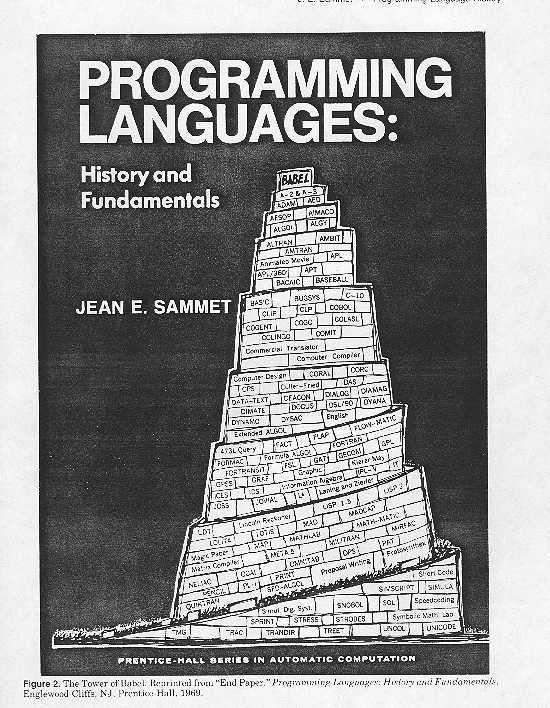
\includegraphics[width=.5\textwidth]{babel}
   \caption{The Babel's Tower of programming languages, taken from the cover of
      J. Sammet's \emph{Programming Languages: History and Fundamentals} (1969).
      Being a 1969 book, the picture misses several important additions,
      nevertheless it is still representative of the difficulty in choosing a
      suitable programming language.
   }
\end{figure}

\section{Glimpse at functional programming languages}
Functional programming languages has gained attraction over imperative ones in recent years due to
their ability to handle effortlessly and in robust way concurrency and
multithreading/multicore 
computing, making them particularly suitable to distributed frameworks. 

Historically, concurrent programming was not the original motivation for
functional programming. 
After the early functional-flavored language Lisp and  the development of APL in the
early 1960s by Iverson, functional programming was eventually formalized by
John Bakus (the father of Fortran) in his
cornerstone 1977 Turing Award Lecture 
\emph{Can Programming Be Liberated From the von Neumann Style?
   A Functional Style and its Algebra of Programs}, where he presented his FP
programming language and emphasizes how liberating a programming language from
the traditional imperative style would have lead to a programming language
closer to mathematical abstractions. 

For several years, functional programming was relegated mainly as an academic
tool. Nevertheless, several powerful functional programming languages have been
developed in the last decades. It is worth mentioning at this point:
Haskell, Erlang, OCam, Closure. 
Scala was build 

\section{Reactive paradigm}

\section{Python}   

\section{IPython  and other notebooks}   
\section{Scala}

\section{Cern ROOT for HEP}
In high-energy physics

\section{Distributed programming: Apache Spark}


\printbibliography[heading=subbibliography]
\end{refsection}

% *****************************************************************************
% Materiale finale
% *****************************************************************************
%*******************************************************
% Bibliografia
%*******************************************************
\cleardoublepage
%\printbibliography
%\printbibheading[heading=bibintoc]
%\bibbysection%[heading = subbibliography]
\printbibheading
\bibbysection[heading=subbibliography]

%
% --- Index ------
%
\cleardoublepage
\manualmark
\markboth{\spacedlowsmallcaps{\indexname}}{\spacedlowsmallcaps{\indexname}}
\phantomsection
\begingroup 
    \let\clearpage\relax
    \let\cleardoublepage\relax
    \let\cleardoublepage\relax
\pagestyle{scrheadings}%???
%\addcontentsline{toc}{chapter}{\numberline{}\tocEntry{\indexname}}
%\mtcaddchapter[\numberline{}\tocEntry{\indexname}]
\printindex
\endgroup 

\end{document}
